\documentclass[11pt, a4paper]{article}\usepackage[]{graphicx}\usepackage[]{xcolor}
% maxwidth is the original width if it is less than linewidth
% otherwise use linewidth (to make sure the graphics do not exceed the margin)
\makeatletter
\def\maxwidth{ %
  \ifdim\Gin@nat@width>\linewidth
    \linewidth
  \else
    \Gin@nat@width
  \fi
}
\makeatother

\definecolor{fgcolor}{rgb}{0.345, 0.345, 0.345}
\newcommand{\hlnum}[1]{\textcolor[rgb]{0.686,0.059,0.569}{#1}}%
\newcommand{\hlsng}[1]{\textcolor[rgb]{0.192,0.494,0.8}{#1}}%
\newcommand{\hlcom}[1]{\textcolor[rgb]{0.678,0.584,0.686}{\textit{#1}}}%
\newcommand{\hlopt}[1]{\textcolor[rgb]{0,0,0}{#1}}%
\newcommand{\hldef}[1]{\textcolor[rgb]{0.345,0.345,0.345}{#1}}%
\newcommand{\hlkwa}[1]{\textcolor[rgb]{0.161,0.373,0.58}{\textbf{#1}}}%
\newcommand{\hlkwb}[1]{\textcolor[rgb]{0.69,0.353,0.396}{#1}}%
\newcommand{\hlkwc}[1]{\textcolor[rgb]{0.333,0.667,0.333}{#1}}%
\newcommand{\hlkwd}[1]{\textcolor[rgb]{0.737,0.353,0.396}{\textbf{#1}}}%
\let\hlipl\hlkwb

\usepackage{framed}
\makeatletter
\newenvironment{kframe}{%
 \def\at@end@of@kframe{}%
 \ifinner\ifhmode%
  \def\at@end@of@kframe{\end{minipage}}%
  \begin{minipage}{\columnwidth}%
 \fi\fi%
 \def\FrameCommand##1{\hskip\@totalleftmargin \hskip-\fboxsep
 \colorbox{shadecolor}{##1}\hskip-\fboxsep
     % There is no \\@totalrightmargin, so:
     \hskip-\linewidth \hskip-\@totalleftmargin \hskip\columnwidth}%
 \MakeFramed {\advance\hsize-\width
   \@totalleftmargin\z@ \linewidth\hsize
   \@setminipage}}%
 {\par\unskip\endMakeFramed%
 \at@end@of@kframe}
\makeatother

\definecolor{shadecolor}{rgb}{.97, .97, .97}
\definecolor{messagecolor}{rgb}{0, 0, 0}
\definecolor{warningcolor}{rgb}{1, 0, 1}
\definecolor{errorcolor}{rgb}{1, 0, 0}
\newenvironment{knitrout}{}{} % an empty environment to be redefined in TeX

\usepackage{alltt}

% Latex packages and options
% =============================================================================
\usepackage{verbatim}
\usepackage[vmargin=3cm, hmargin=2cm, headheight=14pt]{geometry}
\usepackage{url}
\usepackage{hyperref}
\usepackage{fancyhdr}
\usepackage{color}
\usepackage{amsmath, amssymb}
\usepackage{booktabs}
\usepackage{longtable}
\usepackage{lscape}
\usepackage{natbib}
\usepackage{xspace}
% spacing
\linespread{1.05}
% sans serif caption (added by sina)
\usepackage[font=sf, labelfont={sf}, margin=1cm]{caption}
% encodings
\usepackage[T1]{fontenc}
\usepackage[latin1]{inputenc}

\usepackage{colortbl}
\usepackage{xcolor}
\definecolor{lightgray}{gray}{0.9}

\usepackage{graphicx}
\usepackage{float}
\usepackage{caption}


% =============================================================================
\newcommand{\name}{Manuel Pfister}
\newcommand{\mail}{manuel.pfister@uzh.ch}
\newcommand{\versiondate}{\today}
\newcommand{\supervisor}{$<$Supervisor Name$>$}
\newcommand{\projecttitle}{Inferential Seamless Designs for Treatment Selection during a Phase II/III Study in Oncology}
\newcommand{\subtitle}{Master Thesis \\%[.15cm]
  {\Large XYZ} \\[.25cm]
   {\large EBPI, Department of Biostatistics}}

% Headers and footers
% =============================================================================
\fancypagestyle{standard}{
\fancyhf{}
\renewcommand{\footrulewidth}{0.4pt}
\fancyfoot[c]{\thepage}
\fancyfoot[l]{\textsf{\name}, \href{mailto::\mail}{\textsf{\emph{\mail}}}}
\fancyfoot[r]{\textsf{\versiondate}}
\renewcommand{\headrulewidth}{0.4pt}
\fancyhead[c]{}
\fancyhead[r]{\textsf{\inst}}
}

% knitr options
% =============================================================================
% If you use RStudio, make sure set the following option:
% Tools -> Global Options -> Sweave -> Weave Rnw files using: knitr


\IfFileExists{upquote.sty}{\usepackage{upquote}}{}
\begin{document}

% Title Page
\begin{titlepage} % Creates a title page environment
    \centering
    \vspace*{1cm} % Adjust vertical space as needed
    \rule{\linewidth}{1pt}\par\vspace{0.5cm} % Upper horizontal line
    {\LARGE Inferential Seamless Designs for Treatment Selection during a Phase II/III Study in Oncology}
    \vspace{0.5cm}
    \rule{\linewidth}{1pt} % Lower horizontal line
    \vspace{2cm}

    \section*{STA495 Master Thesis}
    \vspace{2.5cm}
    Manuel Pfister\\
    (manuel.pfister@uzh.ch / manuel.pfister@bms.com)\\
    Matriculation Number: 19-659-408\\
    \vspace{2cm}

    Supervised by\\
    Dr. Pierre Colin (pierre.colin@bms.com), Bristol Myers Squibb\\
    PD Dr. Malgorzata Roos (malgorzata.roos@uzh.ch), University of Zurich\\
    \vspace{2cm}

    Version: \today\\
    \vspace{2cm}

    % Center logos at the bottom of the title page
    
\includegraphics[width=120pt]{figure/uzh.png}\hspace{1cm}
\includegraphics[width=220pt]{figure/bms.png}\\
\end{titlepage}


\bigskip

\newpage
\thispagestyle{empty}
\mbox{}
\newpage


\section*{Acknowledgement} \label{sec:Acknowledgement}
% =============================================================================

First and foremost, I would like to express my heartfelt gratitude to Pierre from Bristol Myers Squibb. Pierre has been an invaluable source of support and motivation throughout my Master's thesis. He significantly advanced my statistical skills and provided thoughtful guidance that extended beyond my academic work. Despite my demanding schedule as a football referee, he always made time to support me with my thesis, offering both flexibility and unwavering encouragement. His advice and commitment have consistently inspired me, both professionally and personally.\\

\noindent I would also like to extend my sincere thanks to Maggie from the University of Zurich. Her constant support and readiness to assist were invaluable throughout this process. She always came well-prepared, offering constructive feedback and valuable input that greatly enriched my work. Her expertise and willingness to help made a significant impact on the completion of this thesis.\\

\noindent I am also profoundly grateful to the Master's Program in Biostatistics at the University of Zurich for providing me with such a solid foundation in this fascinating field. This program has not only deepened my knowledge but also broadened my horizons, equipping me with the skills necessary for the challenges ahead.\\

\noindent To both Pierre and Maggie, I am truly thankful for their guidance, time, and encouragement, which have been instrumental in helping me navigate this challenging yet rewarding journey.\\

\vspace{1cm}
\hfill
\begin{minipage}{0.4\textwidth}
\raggedleft
Manuel Pfister\\
December 2024
\end{minipage}

\newpage


\tableofcontents
\newpage


\section*{Abbreviations}

\begin{tabular}{ll}
BMS                  & Bristol Myers Squibb \\
CI                   & Confidence Interval \\
DTL                  & Drop-the-Losers \\
EBPI                 & Epidemiology, Biostatistics and Prevention Institute \\
FWER                 & Family-Wise Error Rate \\
GBDS                 & Global Biostatistics and Data Science \\
HR                   & Hazard Ratio \\
MAMS                 & Multi-Arm Multi-Stage \\
MCSE                 & Monte Carlo Standard Error \\
ORR                  & Objective Response Rate \\
OS                   & Overall Survival \\
PFS                  & Progression-Free Survival \\
R                    & R Programming Language \\
SoC                  & Standard of Care \\
UZH                  & University of Zurich \\
\end{tabular}



\newpage
% =============================================================================
\section*{Abstract} \label{sec:abstract}

In drug development, clinical trials are a cornerstone of evaluating new treatments. However, traditional designs often face significant challenges in efficiency, particularly when assessing multiple treatment options. The emergence of Multi-Arm Multi-Stage (MAMS) designs, such as the "Drop-the-Losers" approach, offers innovative solutions by combining multiple hypotheses within a single trial framework. This thesis evaluates the "Drop-the-Losers" approach, focusing on its application in Phase II/III oncology trials, where identifying promising treatments early is critical.

This work extends existing methodologies by incorporating binary and survival endpoints, addressing limitations of earlier designs which focused primarily on continuous outcomes. Using simulation studies, the statistical performance of the "Drop-the-Losers" design was assessed across diverse clinical scenarios. Key metrics included Type I error control, statistical power and the Monte Carlo Standard Error (MCSE) under varying endpoint distributions. Simulations involved endpoints such as progression-free survival (PFS).

Results demonstrated that the "Drop-the-Losers" design effectively balances statistical rigor and efficiency. The design maintained robust Type I error control while ensuring high power in detecting clinically relevant effects. Scenarios with harmful or ineffective treatments highlighted the ethical advantage of eliminating suboptimal options early, minimizing patient exposure to ineffective therapies.

One limitation identified is that long-term survival endpoints may not be mature enough to support early treatment selection analyses. Updating the endpoint of interest over time could align with clinical practices, starting with objective response rate (ORR) at the first analysis, transitioning to Benefit-Risk scores or PFS at the second analysis, and concluding with overall survival (OS) at the final analysis. However, such an approach requires careful handling of correlations between drug effects across these endpoints, since selecting treatments based on a poor surrogate endpoint.

This thesis provides a comprehensive framework for implementing "Drop-the-Losers" designs in clinical trials, demonstrating its potential to accelerate treatment evaluation in oncology while upholding ethical and scientific standards. This methodology contributes to the ongoing evolution of designs, underscoring their value in modern clinical research.



\newpage
\section{Introduction} \label{sec:intro}
% =============================================================================

Clinical trials are the cornerstone of clinical drug development, playing a critical role in evaluating new treatments, particularly in fields such as oncology where multiple treatment options are often explored concurrently. However, traditional clinical trial designs are often resource-intensive and time-consuming, particularly when multiple treatments need to be tested. Multi-Arm Multi-Stage (MAMS) trial designs, such as the "Drop-the-Losers" (DTL)  approach proposed by \cite{Wason2017DropTheLosers}, provide a more efficient alternative by allowing multiple treatments to be evaluated within the same trial while utilizing interim analyses to drop the less effective or less promising treatments early.

Oncology trials often involve complex decision-making processes, including the evaluation of multiple drug combinations, schedules, and dose levels. The need to efficiently select the most effective treatments early in the trial is critical for improving patient outcomes and expediting the drug development process. Traditional clinical trial designs, which evaluate one treatment at a time, do not address this need effectively due to inefficiencies in time, cost, and sample size requirements. The "Drop-the-Losers" design offers a powerful solution by allowing several treatments to be tested simultaneously, with less promising treatments being dropped at each interim analysis. This design is particularly advantageous in Phase II/III studies, where treatments are first screened for efficacy (excluding safety in this design) and selected for further evaluation in Phase III, even if certain aspects like optimal dose or combinations still require exploration.

This master thesis focuses on evaluating the performance of the "Drop-the-Losers" design in Phase II/III oncology trials, where treatment selection is crucial for determining the most effective therapies for patients. The design is characterized by interim analyses at predefined stages, where a number of experimental treatments are dropped based on their performance relative to a control group. This approach optimizes resource allocation by focusing efforts on more promising treatments while maintaining robust statistical power and controlling Type I error rates. The primary objective of this is to assess the effectiveness of the "Drop-the-Losers" design in controlling Type I error rates and maintaining statistical power while efficiently selecting promising treatments. The study investigates how this design performs under different clinical scenarios involving continuous, binary, and survival endpoints. Additionally, the study will also examine the Monte Carlo standard error (MCSE) associated with the design.

This thesis employs a simulation study to assess the performance of the "Drop-the-Losers" design across various clinical scenarios. Simulations were conducted in the R programming language using parallel computing to manage the computational complexity. While ~\cite{Wason2017DropTheLosers} has already addressed continuous outcomes, this study focuses on extending the DTL approach to binary outcomes, as well as survival outcomes like progression-free survival (PFS), which are essential endpoints in oncology trials. The study evaluates the statistical properties of the design, including Type I error rates, statistical power, and biases under various configurations of treatment effects, such as the null hypothesis and hybrid models with one or more effective treatments.

The Methods section outlines the methodological framework of the "Drop-the-Losers" design, including its mathematical formulation and application to binary and survival endpoints. The Results section presents findings from the simulation study, evaluating the design's performance across various scenarios. The Discussion addresses the implications of these results, highlighting the strengths, limitations, and ethical considerations of the design. Finally, the Conclusion summarizes the key insights and provides recommendations for future research. Additional details and supplementary results are included in the appendices.


\section{Methods} \label{sec:methods}
% =============================================================================

In this section, we present the methods used in this study, focusing on the Multi-Arm Multi-Stage (MAMS) trial design and the "Drop-the-Losers" approach. Additionally, we illustrate the application of these methods with an example using continuous endpoints to demonstrate their practical implementation.


\subsection{Multi-Arm Multi-Stage Study Design}

The MAMS design is an adaptive clinical trial framework that enables the simultaneous evaluation of multiple treatments within a single trial. Unlike traditional designs, which require separate trials for each treatment, MAMS designs incorporate interim analyses at predefined stages to assess treatment efficacy. Treatments that fail to demonstrate sufficient promise are dropped early, allowing resources to focus on the most effective options. This approach improves efficiency, reduces costs, and shortens the time needed to identify successful therapies while maintaining rigorous control over statistical error rates. The MAMS design is particularly useful in settings with limited resources or when rapid treatment evaluation is essential, such as in oncology \citep{Royston2003MAMS}. This study evaluates a MAMS clinical trial design, focusing on the DLT approach as discussed by \cite{Wason2017DropTheLosers}. As shown in Figure~\ref{fig:mams_design}, the MAMS framework, allows multiple experimental treatments to be assessed in parallel within a single trial. At the outset, we have four treatment arms. During each interim analysis, the arms are assessed for futility or high efficacy. In the first interim analysis, treatment arm 2 is removed, and in the second interim analysis, treatment arm 1 is eliminated. By the end, two arms remain, which are compared against the standard of care to determine if they are significantly better.

As with any design incorporating interim analyses, the issue of multiple testing arises, along with the associated risks of Type I and Type II errors. This challenge can be addressed by applying a spending function, such as the Pocock spending function~\citep{spendingFunction}, which allocates the significance level across interim analyses in a controlled manner. Later in this section, the DLT design is introduced, highlighting the differences compared to the traditional MAMS (Multi-Arm Multi-Stage) design.


\begin{figure}[H]
    \centering
    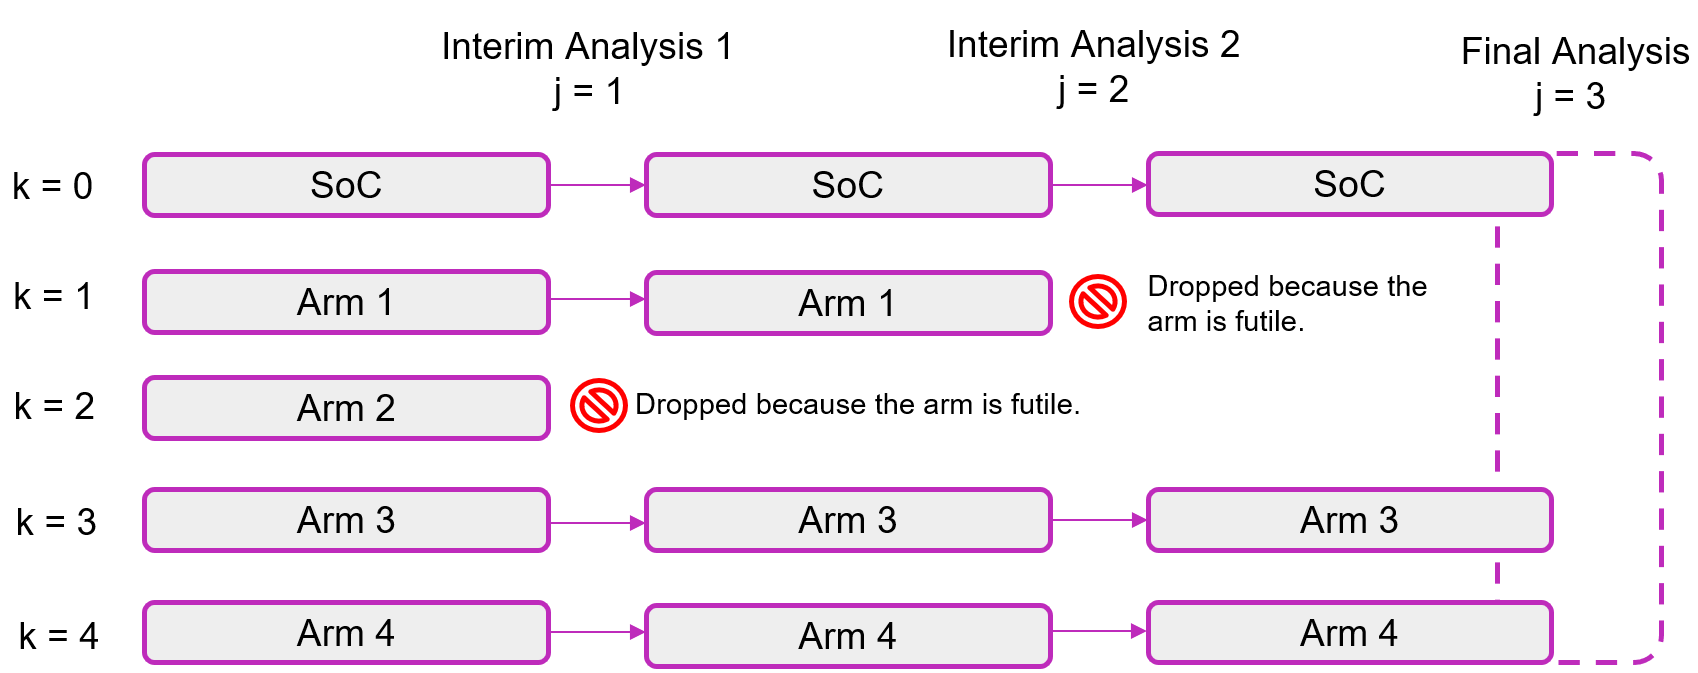
\includegraphics[width=\textwidth]{figure/Mams.png}
    \caption{Illustration of the Multi-Arm Multi-Stage (MAMS) trial design. Treatments are evaluated at each interim analysis. Treatments showing insufficient efficacy (futile) are dropped, while the most promising treatments continue to the next stage. The final analysis compares the remaining treatments to the control (SoC: Standard of Care).}
    \label{fig:mams_design}
\end{figure}


\subsection{Drop-the-Losers Study Design}


In this section, we discuss the specific design of MAMS studies, particularly the Drop-the-Losers (DTL) design, with a focus on hypothesis testing, the distribution of treatment outcomes, and the underlying concept.

At the end of stage $j$, let $Z_j^{(k)}$ be the test statistic~(\ref{eq:Z_j_k}) for treatment $k$. The treatments are ranked according to these statistics, and a fixed number of treatments with the worst test statistics are dropped. Let $n^{(j)}$ represent the number of treatments remaining at stage $j$. The design is defined by the sequence of treatment counts across stages: $K : n^{(2)} : n^{(3)} : \dots : n^{(J)}$, where $n^{(J)} = 1$ (indicating that only one experimental treatment reaches the final stage). At each interim analysis, the least promising treatments are dropped based on their ranked test statistics (see Figure \ref{fig:drop_losers}). The exact number of treatments to be dropped is prespecified, and the remaining treatments proceed to the next stage.

We focus on the 4:2:1 design, which consists of 4 treatment arms, followed by 2 arms in Interim Analysis 2, and finally 1 arm in the final stage. However, any design of the form \(K:L:1\) can be applied, where \(K\) represents the total number of arms, \(L\) is the number of arms at Interim Analysis 2, and 1 corresponds to the single arm in the final analysis.

From a practical perspective, prespecifying the number of treatments to be dropped stabilizes the sample size across stages, which would otherwise be treated as a random variable. Such randomness could lead to significant variability in resource requirements and logistical challenges during trial execution. By ensuring a fixed number of treatments at each stage, the design aligns with the goals of resource-efficient clinical trials while retaining robust statistical rigor. Wason's publication showed, when using a continuous endpoint, that the sample size required by the Drop-the-Losers design is similar to the average sample size required by other MAMS designs. With the Drop-the-Losers design, the future study expenses are no longer considered as a risk ~\citep{Wason2017DropTheLosers}.

The control group remains in the trial throughout all stages. At the final stage, the remaining treatment arm is compared to the control arm, and if its test statistic exceeds a predefined significance threshold \( c \), it is declared superior to the control. The \( c \)-value represents a critical threshold that controls both Type I and Type II errors in hypothesis testing. Type I error (false positive) occurs when the null hypothesis is incorrectly rejected, i.e., when a treatment is declared superior to the control even though no true difference exists. Conversely, Type II error (false negative) occurs when the null hypothesis fails to be rejected, i.e., when a treatment is not declared superior despite a true underlying difference~\ref{bland2015introduction}. The numerical calculation of the test statistic and the corresponding threshold \( c \) will be further discussed in the Results~\ref{sec:simulation_design}.

Let $k \in \{0, 1, \dots, K\}$ index the treatments, with $k=0$ representing the control treatment. The outcome for each patient $i$ on treatment $k$ is denoted by $X_{ki}$, assumed to be normally distributed with mean $\mu_k$ and variance $\sigma^2$. For \( k \in \{0, 1, \dots, K\} \), define \( \delta_k = \mu_k - \mu_0 \). The null hypothesis for each treatment $k$ is $H_0^{(k)}: \mu_k \leq \mu_0$, where $\mu_0$ is the mean outcome for the control group. The alternative hypothesis is $H_1^{(k)}: \mu_k > \mu_0$. The global null hypothesis, $H_0$, is that all treatments are no better than the control, i.e., $\mu_k \leq \mu_0$ for all $k \in \{1, \dots, K\}$. The global alternative hypothesis, $H_1$, is that at least one treatment is better than the control, i.e., $\mu_k > \mu_0$ for at least one $k \in \{1, \dots, K\}$.

At each stage $j$, the test statistic for treatment $k$ is computed as:
\begin{equation}
Z_j^{(k)} = \frac{\frac{1}{n_j}\sum_{i=1}^{n_j} X_{ki} - \frac{1}{n_j}\sum_{i=1}^{n_j} X_{0i}}{\sqrt{2\sigma^2 / n_j}}\label{eq:Z_j_k}
\end{equation}
where $n_j$ is the number of patients observed up to stage $j$. This statistic~(\ref{eq:Z_j_k}) has a marginal distribution $\mathcal{N}\left(\delta_k \cdot \sqrt{\frac{n_j}{2\sigma^2}}, 1\right)$ and the covariance between test statistics at two different stages is given by

\begin{equation}
\text{Cov}(Z_j^{(k)}, Z_l^{(m)}) = \sqrt{\frac{\min(n_j, n_l)}{\max(n_j, n_l)}},\label{eq:covariance1}
\end{equation}

if $k$ = $m$ (same treatment) across stages $j$ and $l$ (different stages), and

\begin{equation}
\text{Cov}(Z_j^{(k)}, Z_l^{(m)}) = \frac{1}{2} \sqrt{\frac{\min(n_j, n_l)}{\max(n_j, n_l)}}, \label{eq:covariance2}
\end{equation}

if $k$ $\neq$ $m$ (different treatment) across stages $j$ and $l$ (different stages)~\citep{Wason2017DropTheLosers}.\\

The correlation~(\ref{eq:covariance1},~\ref{eq:covariance2}) between test statistics arises due to two main reasons: First, the cumulative nature of the data, as information from earlier stages contributes to later stages, and second, the shared control group across treatment arms, which introduces dependencies in the comparisons between different treatments and the control. These factors inherently link the test statistics, making them non-independent across stages and treatments.


\begin{figure}[ht]
    \centering
    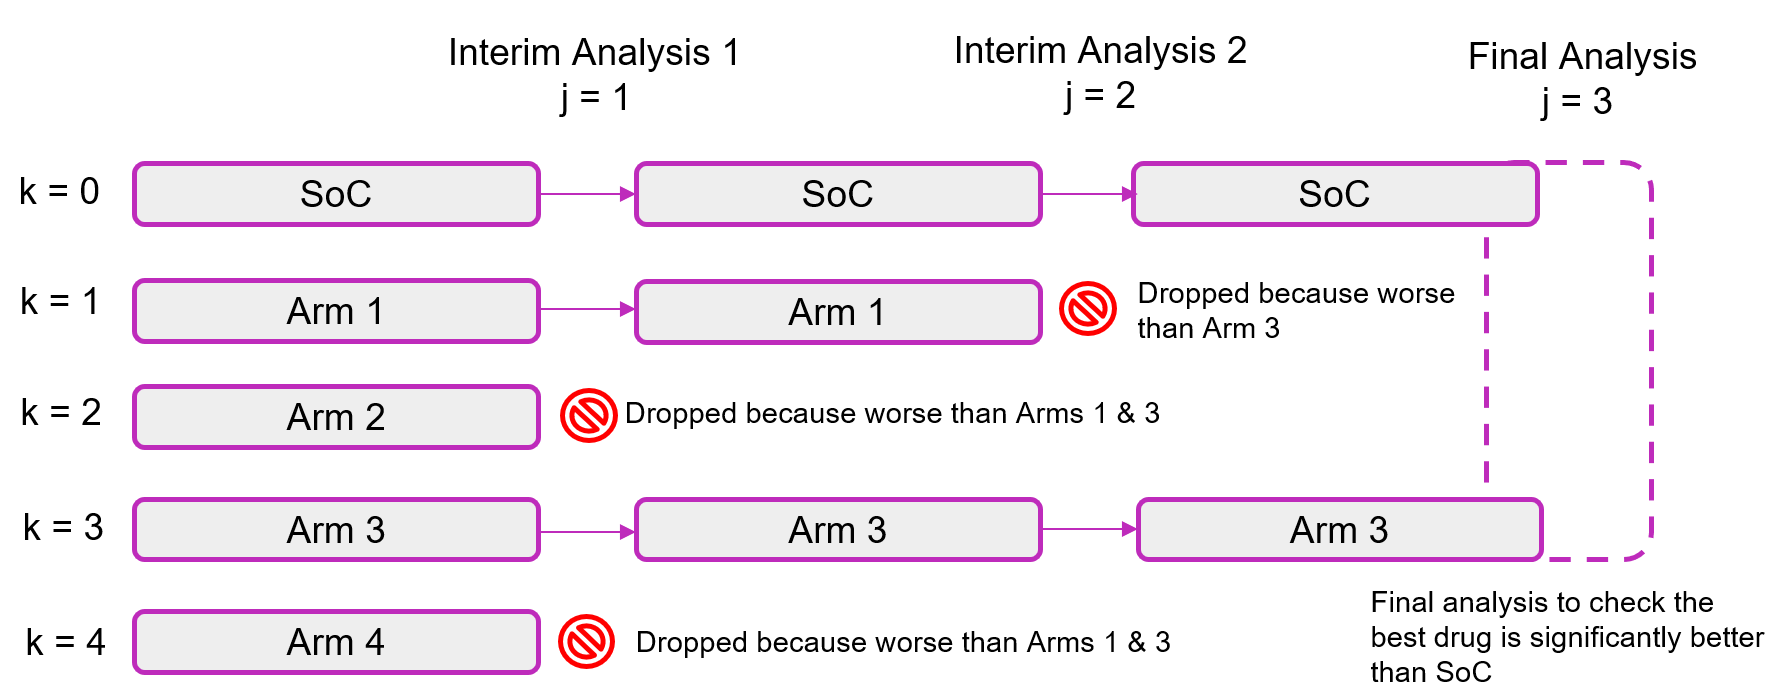
\includegraphics[width=\textwidth]{figure/drop_the_loser.png}
    \caption{Illustration of the (4:2:1) "Drop-the-Losers" design. Treatments are evaluated at each interim analysis. Treatments with the least promising results are dropped, while the most promising treatments continue to the next stage. The process continues until the final analysis, where the remaining treatment is compared to the control.}
    \label{fig:drop_losers}
\end{figure}


\subsection{Analytical Operational Properties} \label{sec:operating_characteristics}

Having outlined the structure and mechanics of the Drop-the-Losers study design, we now explore its analytical operational properties. Specifically, we derive formulas for the probability of recommending a treatment, rejecting the global null hypothesis, and selecting the best treatment under various configurations, particularly focusing on the Least-Favourable-Configuration (LFC) scenario.

For simplicity, the analysis focuses again on a three-stage design with $K$ treatments in the first stage, $L$ in the second, and a remaining candidate in the third stage, which is referred to as a $K:L:1$ design.

\paragraph{Ranking of Treatments}
The probability that a given treatment $k$ is recommended is based on a ranking of the experimental treatments $\psi = (\psi_1, \ldots, \psi_K)$. The following conditions are satisfied for $\psi$:
\begin{enumerate}
    \item The treatment that reaches the final analysis is ranked $1$.
    \item The treatment excluded in an earlier analysis with the lowest test statistic is ranked $K$.
    \item If treatment $k_1$ is excluded later than treatment $k_2$, then $\psi_{k_1} < \psi_{k_2}$.
    \item If treatments $k_1$ and $k_2$ are excluded in the same stage and $k_1$ has a higher test statistic, then $\psi_{k_1} < \psi_{k_2}$.
\end{enumerate}
The probability that $H_0^{(k)}$ is rejected for treatment $k$ is:
\begin{equation}
P(\text{Reject } H_0^{(k)} | \delta) = P(\psi_k = 1, Z^{(k)} > c | \delta),
\end{equation}
where $Z^{(k)}$ is the test statistic for treatment $k$ in the final stage, and $c$ is the critical value.

\paragraph{Multivariate Normal Distribution and Matrix Representation}
The distribution of the test statistics $Z = (Z^{(1)}, Z^{(2)}, \ldots, Z^{(K)})$ is multivariate normal, with the mean $m(\delta)$ and the covariance matrix $\Sigma$ determined by the effects $\delta$ and the study design. For a given ranking $\psi$, the probabilities can be reformulated into conditions on pairwise elements of the test statistic $Z$:
\begin{equation}
(AZ)_i > 0 \quad \forall i,
\end{equation}
where $A$ is a matrix defining the differences and critical values in the ranking. For an example with a $4:2:1$ design, the matrix $A$ is:
\[
A =
\begin{bmatrix}
0 & 1 & 0 & 0 & 1 & 0 & -1 & 0 \\
0 & 0 & 0 & 1 & -1 & 0 & 0 & 0 \\
\vdots & & & \vdots & & & & \vdots \\
0 & 0 & 1 & 0 & 0 & -1 & 0 & 0
\end{bmatrix}.
\]

\paragraph{Probability of Treatment Recommendation under the LFC}
For the Least-Favourable-Configuration scenario, it is assumed that the treatment effect for a reference treatment $\delta^{(1)}$ is clinically relevant, while all other effects $\delta^{(k)}$ ($k = 2, \ldots, K$) are considered negligible. The probability that the reference treatment $k = 1$ is recommended is derived as:
\begin{equation}
(K-1)! \cdot P(\psi_1 = 1, \psi_2 = 2, \ldots, \psi_K = K, Z^{(1)} > c | \delta_1 = \delta^{(1)}, \delta_2 = \delta_3 = \ldots = \delta_K = \delta^{(0)}),
\end{equation}
where $P$ is the marginal probability of a multivariate normal distribution.


\subsection{Step-by-Step Example: 4:2:1 DTL for Continuous Endpoints}

The following example is a fictional scenario designed to illustrate the application of a 4:2:1 Drop-the-Loser design for continuous endpoints. All parameters and calculations are hypothetical and do not represent any real-world clinical trial data.
\begin{itemize}
    \item Number of treatment arms: \( K = 4 \) (\( k = 1, 2, 3, 4 \)).
    \item Control arm: \( k = 0 \).
    \item Number of stages: \( J = 3 \), with 2 interim analyses and 1 final analysis.
    \item Group sizes at each stage:
          \[
          n_1 = 20, \quad n_2 = 40, \quad n_3 = 60.
          \]
\end{itemize}


\begin{table}[h!]
    \centering
    \begin{tabular}{|c|c|c|c|}
    \hline
    \rowcolor[gray]{0.9} \textbf{Arms} & \textbf{Interim Analysis 1 (j=1)} & \textbf{Interim Analysis 2 (j=2)} & \textbf{Final Analysis (j=3)} \\
    \hline
    \text{Control (k=0)} & 1.0 & 1.0 & 1.0 \\
    \text{Treatment 1 (k=1)} & 1.5 & 1.7 & \text{Dropped} \\
    \text{Treatment 2 (k=2)} & 1.2 & \text{Dropped} & \text{Dropped} \\
    \text{Treatment 3 (k=3)} & 1.3 & 1.6 & 1.8 \\
    \text{Treatment 4 (k=4)} & 1.1 & \text{Dropped} & \text{Dropped} \\
    \hline
    \end{tabular}
    \caption{Overview of the treatment effects at each stage and the final analysis.}
    \label{tab:example}
\end{table}

\paragraph{Test Statistics, Covariance, and Contrast Matrices}\\

\subparagraph{Test Statistics for Interim Analysis 1:}
The test statistic for each treatment arm at Interim Analysis 1 is:
\[
Z_1^{(k)} = \left( \frac{\sum_{i=1}^{n_1} X_{ki}}{n_1} - \frac{\sum_{i=1}^{n_1} X_{0i}}{n_1} \right) \sqrt{\frac{n_1}{2\sigma^2}}.
\]
Using the observed means from Interim Analysis 1 from the Table~\ref{tab:example}:

\begin{equation}
Z_1^{(1)} = \left( \frac{1.5}{20} - \frac{1.0}{20} \right) \sqrt{\frac{20}{2 \cdot 1}} = 0.079,
\end{equation}

\begin{equation}
Z_1^{(2)} = \left( \frac{1.2}{20} - \frac{1.0}{20} \right) \sqrt{\frac{20}{2 \cdot 1}} = 0.032,
\end{equation}

\begin{equation}
Z_1^{(3)} = \left( \frac{1.3}{20} - \frac{1.0}{20} \right) \sqrt{\frac{20}{2 \cdot 1}} = 0.047,
\end{equation}

\begin{equation}
Z_1^{(4)} = \left( \frac{1.1}{20} - \frac{1.0}{20} \right) \sqrt{\frac{20}{2 \cdot 1}} = 0.016.
\end{equation}



\paragraph{Test Statistics for Interim Analysis 2}
The test statistic for each treatment arm at Interim Analysis 2 is:
\[
Z_2^{(k)} = \left( \frac{\sum_{i=1}^{n_2} X_{ki}}{n_2} - \frac{\sum_{i=1}^{n_2} X_{0i}}{n_2} \right) \sqrt{\frac{n_2}{2\sigma^2}}.
\]
Using the observed means from Interim Analysis 2 from Table~\ref{tab:example}, we compute:
\begin{equation}
Z_2^{(1)} = \left( \frac{1.7}{40} - \frac{1.0}{40} \right) \sqrt{\frac{40}{2 \cdot 1}} = 3.13,
\end{equation}

\begin{equation}
Z_2^{(3)} = \left( \frac{1.6}{40} - \frac{1.0}{40} \right) \sqrt{\frac{40}{2 \cdot 1}} = 2.68. \label{eq:Z2_3}
\end{equation}

Treatment arms \(k=2\) and \(k=4\) were dropped at this stage.

\paragraph{Test Statistics for Final Analysis}
The test statistic for each remaining treatment arm at the Final Analysis is
\[
Z_3^{(k)} = \left( \frac{\sum_{i=1}^{n_3} X_{ki}}{n_3} - \frac{\sum_{i=1}^{n_3} X_{0i}}{n_3} \right) \sqrt{\frac{n_3}{2\sigma^2}}.
\]
Using the observed means from the Final Analysis from Table~\ref{tab:example}, we compute:
\begin{equation}
Z_3^{(3)} = \left( \frac{1.8}{60} - \frac{1.0}{60} \right) \sqrt{\frac{60}{2 \cdot 1}} = 4.38.
\end{equation}

Treatment arms \(k=1\), \(k=2\), and \(k=4\) were dropped prior to the Final Analysis.






\paragraph{Contrast Matrix}\\

The contrast matrix \( A \) is used to define the pairwise comparisons between treatment arms and the control in a 4:2:1 "Drop-the-Losers" design. The matrix accounts for dropping \( k = 2 \) and \( k = 4 \) after the first interim analysis and \( k = 1 \) after the second interim analysis, as observed in the means provided and further illustrated in Equations~\eqref{eq:Z1_2} and~\eqref{eq:Z1_4}. This results in only \( k = 3 \) proceeding to the final analysis. The matrix is defined as

\begin{equation}
\setlength{\arraycolsep}{3pt}
A =
\left[
\begin{array}{cccccccccccc}
0 & 0 & 0 & 1 & 0 & 0 & 0 & 0 & 0 & -1 & 0 & 0 \\
1 & 0 & 0 & -1 & 0 & 0 & 0 & 0 & 0 & 0 & 0 & 0 \\
0 & 0 & -1 & 0 & 0 & 1 & 0 & 0 & 0 & 0 & 0 & 0 \\
0 & -1 & 0 & 0 & 0 & 0 & 0 & 1 & 0 & 0 & 0 & 0 \\
0 & 0 & 0 & 0 & 0 & 0 & 0 & 0 & 1 & 0 & 0 & 0
\end{array}
\right]. \label{eq:contrast_matrix}
\end{equation}


\begin{flushleft}
\textbf{Row 1}: Compares \( Z_1^{(4)} \) with \( Z_1^{(2)} \), indicating that Arm 4 performs worse than Arm 2.\\
\textbf{Row 2}: Compares \( Z_1^{(2)} \) with \( Z_1^{(1)} \), indicating that Arm 2 performs worse than Arm 1.\\
\textbf{Row 3}: Compares \( Z_1^{(3)} \) with \( Z_1^{(1)} \), indicating that Arm 1 performs worse than Arm 2.\\
\textbf{Row 4}: Compares \( Z_2^{(1)} \) with \( Z_2^{(3)} \), indicating that Arm 1 performs worse than Arm 3.\\
\textbf{Row 5}: Tests whether \( Z_3^{(3)} \), the remaining arm in the final analysis, is significantly better than the control.
\end{flushleft}


The contrast vector \( C \) is obtained by multiplying the contrast matrix \( A \)~(\ref{eq:contrast_matrix}) with the vector of test statistics \( Z \)~(\ref{eq:Z_stages}). The test statistics vector \( Z \) contains all test statistics for the treatment arms (\( k = 1, 2, 3, 4 \)) across all stages (\( j = 1, 2, 3 \)):

\begin{equation}
Z =
\begin{bmatrix}\label{eq:Z_stages}
Z_1^{(1)} \\ Z_2^{(1)} \\ Z_3^{(1)} \\
Z_1^{(2)} \\ Z_2^{(2)} \\ Z_3^{(2)} \\
Z_1^{(3)} \\ Z_2^{(3)} \\ Z_3^{(3)} \\
Z_1^{(4)} \\ Z_2^{(4)} \\ Z_3^{(4)}
\end{bmatrix}.
\end{equation}


\paragraph{Step-by-Step Multiplication:}
Using the contrast matrix \( A \) and the test statistics vector \( Z \), the contrast vector \( C \) is computed. Each element of \( C \) represents a specific contrast derived from the matrix multiplication \( C = A \cdot Z \). For example:

\[
C_1 = 0 \cdot Z_1^{(1)} + 0 \cdot Z_2^{(1)} + 0 \cdot Z_3^{(1)} + 1 \cdot Z_1^{(2)} + 0 \cdot Z_2^{(2)} + 0 \cdot Z_3^{(2)} + 0 \cdot Z_1^{(3)} + 0 \cdot Z_2^{(3)} + 0 \cdot Z_3^{(3)} - 1 \cdot Z_1^{(4)} + 0 \cdot Z_2^{(4)} + 0 \cdot Z_3^{(4)}.
\]

This simplifies to:
\[
C_1 = Z_1^{(2)} - Z_1^{(4)}.
\]

Similarly, the remaining contrasts are computed as follows:

\[
C_2 = 1 \cdot Z_1^{(1)} + 0 \cdot Z_2^{(1)} + 0 \cdot Z_3^{(1)} - 1 \cdot Z_1^{(2)} + 0 \cdot Z_2^{(2)} + 0 \cdot Z_3^{(2)} + 0 \cdot Z_1^{(3)} + 0 \cdot Z_2^{(3)} + 0 \cdot Z_3^{(3)} + 0 \cdot Z_1^{(4)} + 0 \cdot Z_2^{(4)} + 0 \cdot Z_3^{(4)}.
\]

This simplifies to:
\[
C_2 = Z_1^{(1)} - Z_1^{(2)}.
\]

\[
C_3 = 0 \cdot Z_1^{(1)} + 0 \cdot Z_2^{(1)} - 1 \cdot Z_3^{(1)} + 0 \cdot Z_1^{(2)} + 1 \cdot Z_2^{(2)} + 0 \cdot Z_3^{(2)} + 0 \cdot Z_1^{(3)} + 0 \cdot Z_2^{(3)} + 0 \cdot Z_3^{(3)} + 0 \cdot Z_1^{(4)} + 0 \cdot Z_2^{(4)} + 0 \cdot Z_3^{(4)}.
\]

This simplifies to:
\[
C_3 = Z_2^{(2)} - Z_3^{(1)}.
\]

\[
C_4 = 0 \cdot Z_1^{(1)} - 1 \cdot Z_2^{(1)} + 0 \cdot Z_3^{(1)} + 0 \cdot Z_1^{(2)} + 0 \cdot Z_2^{(2)} + 0 \cdot Z_3^{(2)} + 0 \cdot Z_1^{(3)} + 1 \cdot Z_2^{(3)} + 0 \cdot Z_3^{(3)} + 0 \cdot Z_1^{(4)} + 0 \cdot Z_2^{(4)} + 0 \cdot Z_3^{(4)}.
\]

This simplifies to:
\[
C_4 = Z_2^{(3)} - Z_2^{(1)}.
\]

\[
C_5 = 0 \cdot Z_1^{(1)} + 0 \cdot Z_2^{(1)} + 0 \cdot Z_3^{(1)} + 0 \cdot Z_1^{(2)} + 0 \cdot Z_2^{(2)} + 0 \cdot Z_3^{(2)} + 0 \cdot Z_1^{(3)} + 0 \cdot Z_2^{(3)} + 1 \cdot Z_3^{(3)} + 0 \cdot Z_1^{(4)} + 0 \cdot Z_2^{(4)} + 0 \cdot Z_3^{(4)}.
\]

This simplifies to:
\[
C_5 = Z_3^{(3)}.
\]

Substitute the computed test statistics:
\[
Z =
\begin{bmatrix}
0.079 \\ 0.032 \\ 0.047 \\
3.13 \\ \text{Dropped} \\ 2.68 \\
\text{Dropped} \\ 4.38 \\ \text{Dropped} \\
0.016 \\ \text{Dropped} \\ \text{Dropped}
\end{bmatrix}.
\]

\paragraph{Resulting Contrast Vector:}
Substitute \( Z \) into \( C = A \cdot Z \):
\[
C =
\begin{bmatrix}
C_1 \\ C_2 \\ C_3 \\ C_4 \\ C_5
\end{bmatrix}
=
\begin{bmatrix}
3.13 - 0.016 \\
0.079 - 3.13 \\
2.68 - 0.047 \\
4.38 - 0.032 \\
4.38
\end{bmatrix}.
\]

Perform the calculations:
\[
C =
\begin{bmatrix}
3.114 \\
-3.051 \\
2.633 \\
4.348 \\
4.38
\end{bmatrix}.
\]

\paragraph{Interpretation:}
\begin{itemize}
    \item \( C_1 = 3.114 \): Indicates that Treatment 1 performed much better at Interim Analysis 2 compared to Treatment 4 at Interim Analysis 1.
    \item \( C_2 = -3.051 \): Indicates that Treatment 1 at Interim Analysis 1 performed much worse than at Interim Analysis 2.
    \item \( C_3 = 2.633 \): Indicates that Treatment 2 at Interim Analysis 2 performed better than Treatment 3 at Interim Analysis 1.
    \item \( C_4 = 4.348 \): Indicates that Treatment 3 at Final Analysis performed significantly better than Treatment 2 at Interim Analysis 1.
    \item \( C_5 = 4.38 \): Indicates the absolute performance of Treatment 3 at the Final Analysis compared to the control.
\end{itemize}



\paragraph{Covariance Matrix Calculation}\\
The covariance matrix is not directly used in the calculations shown in this example. However, it plays a crucial role in determining the critical value \(c\) at final analysis and can also be used as a verification in simulation studies. For simplicity, the mathematical derivation is presented in a simplified manner.


The covariance between test statistics for treatment arms \( k \) and \( m \) across stages \( j \) and \( p \) is given by the formulas~\label{eq:covariance1} and~\label{eq:covariance2}.


\nointend\subparagraph{Example: Covariance Matrix for a 4:2:1 Design}\\
For \( n_1 = 20 \), \( n_2 = 40 \), and \( n_3 = 60 \), the covariance matrix \( \Sigma \) for all treatment arms (\( k = 1, 2, 3, 4 \)) across all stages (\( j = 1, 2, 3 \)) is computed as follows:

\paragraph{Step 1: Define the Matrix Structure}
The covariance matrix has dimensions \( (K \cdot J) \times (K \cdot J) \), where \( K = 4 \) (number of treatment arms) and \( J = 3 \) (number of stages). This results in a \( 12 \times 12 \) matrix.

\paragraph{Step 2: Populate Blocks}
1. \textbf{Diagonal blocks (\( k = m \)):} The covariance between the same treatment arm across different stages is:
   \[
   \text{Cov}(Z_j^{(k)}, Z_p^{(k)}) = \sqrt{\frac{\min(n_j, n_p)}{\max(n_j, n_p)}}, \quad p \geq j.
   \]
   For example:
   \( \text{Cov}(Z_1^{(1)}, Z_2^{(1)}) = \sqrt{\frac{20}{40}} = 0.707 \),
   \( \text{Cov}(Z_2^{(1)}, Z_3^{(1)}) = \sqrt{\frac{40}{60}} = 0.816 \).

2. \textbf{Off-diagonal blocks (\( k \neq m \)):} The covariance between different treatment arms is:
   \[
   \text{Cov}(Z_j^{(k)}, Z_p^{(m)}) = \frac{1}{2} \sqrt{\frac{\min(n_j, n_p)}{\max(n_j, n_p)}}, \quad p \geq j.
   \]
   For example:
   \( \text{Cov}(Z_1^{(1)}, Z_2^{(2)}) = \frac{1}{2} \sqrt{\frac{20}{40}} = 0.354 \),
   \( \text{Cov}(Z_2^{(1)}, Z_3^{(2)}) = \frac{1}{2} \sqrt{\frac{40}{60}} =  0.408\).\\

\paragraph{Step 3: Full Covariance Matrix}
Using the formula above, the complete \( 12 \times 12 \) covariance matrix is:

\[
\Sigma =
\renewcommand{\arraystretch}{1.2} % Vertikalen Abstand anpassen
\setlength{\arraycolsep}{2pt} % Horizontalen Abstand anpassen
\left[
\begin{array}{cccccccccccc}
1.000 & 0.707 & 0.577 & 0.500 & 0.354 & 0.289 & 0.500 & 0.354 & 0.289 & 0.500 & 0.354 & 0.289 \\
\cdots & 1.000 & 0.816 & 0.354 & 0.500 & 0.408 & 0.354 & 0.500 & 0.408 & 0.354 & 0.500 & 0.408 \\
\cdots & \cdots & 1.000 & 0.289 & 0.408 & 0.500 & 0.289 & 0.408 & 0.500 & 0.289 & 0.408 & 0.500 \\
\cdots & \cdots & \cdots & 1.000 & 0.707 & 0.577 & 0.500 & 0.354 & 0.289 & 0.500 & 0.354 & 0.289 \\
\cdots & \cdots & \cdots & \cdots & 1.000 & 0.816 & 0.354 & 0.500 & 0.408 & 0.354 & 0.500 & 0.408 \\
\cdots & \cdots & \cdots & \cdots & \cdots & 1.000 & 0.289 & 0.408 & 0.500 & 0.289 & 0.408 & 0.500 \\
\cdots & \cdots & \cdots & \cdots & \cdots & \cdots & 1.000 & 0.707 & 0.577 & 0.500 & 0.354 & 0.289 \\
\cdots & \cdots & \cdots & \cdots & \cdots & \cdots & \cdots & 1.000 & 0.816 & 0.354 & 0.500 & 0.408 \\
\cdots & \cdots & \cdots & \cdots & \cdots & \cdots & \cdots & \cdots & 1.000 & 0.289 & 0.408 & 0.500 \\
\cdots & \cdots & \cdots & \cdots & \cdots & \cdots & \cdots & \cdots & \cdots & 1.000 & 0.707 & 0.577 \\
\cdots & \cdots & \cdots & \cdots & \cdots & \cdots & \cdots & \cdots & \cdots & \cdots & 1.000 & 0.816 \\
\cdots & \cdots & \cdots & \cdots & \cdots & \cdots & \cdots & \cdots & \cdots & \cdots & \cdots & 1.000 \\
\end{array}
\right]
\]\\


\textbf{The interpretation is as follows:} The diagonal elements of the matrix represent the variance of the test statistics for the same treatment arm at the same stage, with
$\text{Var}(Z_j^{(k)}) = 1.0$. The off-diagonal elements indicate the covariance between test statistics. Higher covariance values are observed for stages that are closer together, due to a larger ratio of $\frac{n_j}{n_p}$. Additionally, the covariance is halved for test statistics from different treatment arms ($k \neq m$).



\paragraph{Calculation of the Critical Value \( c \)}\\

The critical value \( c \) is determined to control the family-wise error rate (FWER) at the specified level \( \alpha = 0.05 \). This ensures that the probability of at least one false positive across all tests does not exceed \( \alpha \).

\subparagraph{Numerical Calculation}\\
Using the provided R code, the critical value is calculated based on the specified parameters:
\begin{itemize}
    \item \( J = 3 \): Number of stages.
    \item \( K = 4 \): Number of treatment arms.
    \item \( \alpha = 0.05 \): Family-wise error rate.
    \item Covariance matrix \( \Sigma \): As defined earlier.
    \item Contrast matrix \( A \): As defined earlier.
\end{itemize}

The calculation in R uses the following function:

\begin{verbatim}

# Function to calculate the integral of the Type I error
integral_typeIerror <- function(c, requiredtypeIerror, mean, var, K) {
  lower <- rep(0, length(mean))
  lower[length(lower)] <- c
  upper <- rep(Inf, length(mean))
  int <- pmvnorm(lower = lower, upper = upper, mean = mean, sigma = var)
  return(as.double(int) * factorial(K) - requiredtypeIerror)
}

c <- uniroot(integral_typeIerror, lower = -2, upper = 5,
             requiredtypeIerror = 0.05, mean = A %*% mu,
             var = A %*% Sigma %*% t(A))$root
\end{verbatim}

\subparagraph{Resulting Critical Value}\\
The calculated critical value is:
\[
c = 1.906.
\]

\subparagraph{Application of the Critical Value}\\

The critical value \( c = 1.906 \) is applied to the final stage of the trial to determine significance:
\begin{itemize}
    \item If the test statistic \( Z_j^{(k)} > c \), the treatment \( k \) is deemed significantly better than the control.
    \item In this example, for \( k = 3 \), the final test statistic is \( Z_3^{(3)} = 4.38 \), which satisfies \( Z_3^{(3)} > c \). Thus, treatment \( k = 3 \) is significantly better than the control.
\end{itemize}

\subparagraph{Conclusion}\\
By applying the critical value \( c = 1.906 \), we conclude that treatment \( k = 3 \) is significantly better than the control in the final analysis. All other treatments were dropped at earlier stages based on the interim analyses.



\newpage
\section{Results: Derivations} \label{sec:results_derivation}
% =============================================================================

\subsection{Binary Outcomes}
For binary outcomes, we assume the response variable follows a binomial distribution, and the test statistic is computed based on the proportion of successes. The test statistic for binary outcomes at stage $j$ is:
\begin{equation}
Z_j^{(k)} = \frac{\sum_{i=1}^{n_j} (X_{ki} - X_{0i})}{\sqrt{2p(1 - p) n_j}}
\end{equation}
The covariance between test statistics for binary outcomes across different stages is given by:
\begin{equation}
\text{Cov}(Z_j^{(k)}, Z_l^{(m)}) = \sqrt{\frac{p(1 - p)}{n_j n_l}} \label{eq:bin_covariance1}
\end{equation}
for $k = m$, and
\begin{equation}
\text{Cov}(Z_j^{(k)}, Z_l^{(m)}) = \frac{1}{2} \sqrt{\frac{p(1 - p)}{n_j n_l}}
\end{equation}
for $k \neq m$. Detailed derivations for binary outcomes can be found in Appendix \ref{sec:app_derivations_binary}.

\subsection{Survival Outcomes}\label{sec:survival_outcomes}
For survival outcomes, we assume a Cox proportional hazards model is applied, and the test statistic is based on the log hazard ratio between the treatment and control arms. The test statistic at stage $j$ is:
\begin{equation}
Z_j^{(k)} \approx \frac{\log \widehat{HR}_{kj}}{\sqrt{\frac{4}{d_j^{(o)} + d_j^{(k)}}}} = \log \widehat{HR}_{kj} \cdot \sqrt{\frac{d_j^{(o)} + d_j^{(k)}}{4}}
\end{equation}
where $\widehat{HR}_{kj}$ is the estimated hazard ratio for treatment $k$ at stage $j$, $d_j^{(o)}$ represents the number of events in the control group, and $d_j^{(k)}$ is the number of events in the treatment group. This statistic assumes that $d_j^{(o)} > d_j^{(k)}$ and adjusts for the number of observed events.

The covariance between test statistics for survival outcomes across different stages $j$ and $p$ is given by
\begin{equation}
\text{Cov}(Z_j^{(k)}, Z_p^{(m)}) = \sqrt{\frac{d_j^{(o)} + d_j^{(k)}}{d_p^{(o)} + d_p^{(k)}}}\label{eq:survival_covariance1},
\end{equation}

for $k = m$ (same treatment arm), and

\begin{equation}
\text{Cov}(Z_j^{(k)}, Z_p^{(m)}) = \frac{1}{2} \sqrt{\frac{d_j^{(o)} + d_j^{(k)}}{d_p^{(o)} + d_p^{(k)}}}\label{eq:survival_covariance2},
\end{equation}

for $k$ $\neq$ $m$ (for different treatment arms).\\


This formula, along with further derivations, is discussed in Appendix \ref{sec:app_derivations_survival}.


\newpage
\section{Results: Simulation Study} \label{sec:simulation_results}
% =============================================================================

The present simulation study adopts the ADEMP framework to systematically evaluate the performance of the 4:2:1 "Drop-the-Losers" design in Phase II and Phase III clinical trial settings. This structured approach ensures transparency and reproducibility while providing insights into the behavior of the design across varying clinical scenarios~\citep{Morris2019}.


\subsection{Design of the Simulation Study} \label{sec:simulation_design}


\begin{figure}[H]
    \centering
    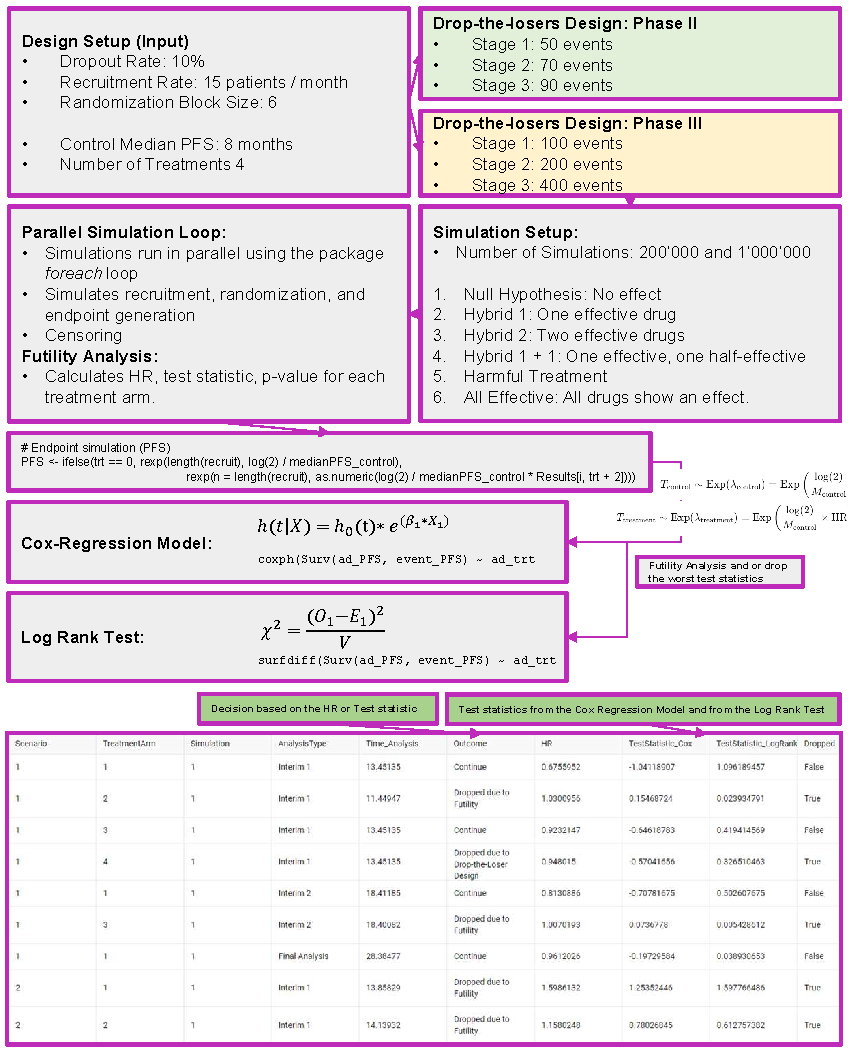
\includegraphics[width=0.85\textwidth]{figure/flowchart_simulation.pdf}
    \caption{Overview of the simulation workflow for the 4:2:1 "Drop-the-Losers" design, including design inputs, simulation structure, and statistical analysis for Phase II and III.}
    \label{fig:simulation_flowchart}
\end{figure}

% AIM

The aim of this simulation study is to evaluate the performance of the 4:2:1 'Drop-the-Losers'(DLT) design in Phase II and Phase III clinical trial settings with survival endpoints (PFS). The primary focus is on controlling the family-wise error rate (FWER) and ensuring sufficient statistical power across various clinical scenarios. These scenarios include both null and alternative hypotheses, where treatment effects of varying magnitudes are considered. The study aims to assess the ability of the design to detect treatment effects, including beneficial effects (hazard ratio \(HR < 1\)), harmful effects (\(HR > 1\)), and scenarios with multiple effective treatments. Furthermore, the study investigates the ethical advantage of dropping harmful arms early in the trial, thus reducing patient exposure to ineffective or harmful treatments.

% Data Generation and Design
The simulation study was designed to mimic the progression of oncology clinical trials utilizing a survival endpoint, specifically progression-free survival (PFS). Survival times for patients were modeled using exponential distributions, where the hazard rates were determined by the baseline hazard and the hypothesized hazard ratios (HRs) for each treatment arm. The hazard ratio represents the relative risk of an event occurring in a treatment arm compared to the control arm. Scenarios included the null hypothesis (\(HR = 1.00\)) as well as alternative hypotheses with varying degrees of treatment efficacy (\(HR < 1.00\)) or harm (\(HR > 1.00\)). Patients were recruited iteratively and randomized into treatment arms using a block randomization scheme to ensure balanced allocation. Recruitment rates and total sample sizes varied between Phase II and Phase III trials to reflect realistic clinical settings. For Phase II trials, event thresholds for interim analyses were set at 30 and 50 cumulative events, with a final analysis at 100 events. For Phase III trials, the thresholds were increased to 100, 200, and 400 events for the two interim analyses and final analysis, respectively. Dropout was incorporated using a censoring mechanism, where patients who left the trial before experiencing an event were treated as censored at their time of dropout. The dropout rate was set to remain constant across all treatment arms to reflect typical clinical practice. Additionally, a two-month delay between interim analyses was introduced to account for practical challenges such as data collection and processing.

To evaluate the futility of treatment arms, Cox proportional hazards models were applied at each interim analysis. Arms deemed futile based on pre-specified thresholds were dropped according to the "Drop-the-Losers" 4:2:1 design. In this case, arms with a hazard ratio (HR) greater than 1.0 were considered futile and dropped, indicating that the treatment arm performed worse than the control or reference treatment. For the final analysis, statistical significance was assessed using test statistics from either the Cox proportional hazards regression model or the log-rank test. A treatment arm was deemed significant if its test statistic exceeded the critical value, which was derived numerically to control the family-wise error rate (FWER). The critical values used were \(c = 2.038\) for Phase II studies (\(\alpha = 0.05\)) and \(c = 2.338\) for Phase III studies (\(\alpha = 0.025\)). The calculated thresholds can be directly applied to the Cox regression test statistics. For the log-rank test, however, the critical value must be squared, as the log-rank test statistic follows a chi-squared distribution under the null hypothesis.

\begin{verbatim}
finddesign_survival(
    J = 3, K = 4, ns = c(4, 2, 1),
    delta1 = 0.5, delta0 = 0.0,
    requiredfwer = 0.025, requiredpower = 0.8,
    groupsizes = c(1, 2/3, 5/3), events = events)
\end{verbatim}

The simulation was implemented in the \texttt{R} programming language using the \texttt{simulate\_trial} and \texttt{simulate\_trial\_log\_rank} functions. The \texttt{doParallel}~\citep{doParallel} package was employed to parallelize the computations, enabling the generation of \(n = 200,000\) simulation runs for each scenario. These runs provided robust estimates of the performance measures, including statistical power, Type I error rates, and the ability to correctly identify effective treatment arms while dropping ineffective or harmful arms at early stages.

The clinical scenarios, detailed in Table~\ref{tab:hazard_ratios}, covered a broad range of treatment effects, from null effects (all \(HR = 1.00\)) to multiple effective arms (\(HR < 1.00\)) or harmful arms (\(HR > 1.00\)). This range allowed a comprehensive assessment of the 4:2:1 design under realistic clinical conditions, ensuring the robustness and adaptability of the simulation framework.


\begin{table}[H]
    \centering
    \caption{Hazard ratios for different treatment arms under various scenarios.}
    \label{tab:hazard_ratios}
    \begin{tabular}{|c|c|c|c|c|}
        \hline
        \rowcolor{gray!20}
        \textbf{Scenario} & \textbf{Arm 1} & \textbf{Arm 2} & \textbf{Arm 3} & \textbf{Arm 4} \\ \hline
        Null Hypothesis & 1.00 & 1.00 & 1.00 & 1.00 \\ \hline
        Hybrid 1        & 0.67 & 1.00 & 1.00 & 1.00 \\ \hline
        Hybrid 2        & 0.67 & 0.67 & 1.00 & 1.00 \\ \hline
        Hybrid 1 + 1    & 0.67 & 0.80 & 1.00 & 1.00 \\ \hline
        Harmful         & 1.20 & 1.00 & 1.00 & 1.00 \\ \hline
        All Effective   & 0.67 & 0.67 & 0.67 & 0.67 \\ \hline
    \end{tabular}
\end{table}

% estimands

The primary estimands of interest in this simulation study were defined to align with the objectives of clinical trials utilizing the 4:2:1 "Drop-the-Losers" design. These estimands focus on characterizing the treatment effect on progression-free survival (PFS) across the different clinical scenarios outlined in Table~\ref{tab:hazard_ratios}.

\begin{itemize}
    \item \textbf{Treatment Effect Estimand:} The relative treatment effect for each experimental arm compared to the control arm was estimated using the hazard ratio (HR). The HR represents the relative risk of progression or death in the experimental arm compared to the control arm. A hazard ratio of 1.00 indicates no effect, whereas a value less than 1.00 suggests a beneficial treatment effect, and a value greater than 1.00 indicates harm.
    \item \textbf{Family-Wise Error Rate (FWER):} The probability of making at least one Type I error (incorrectly declaring a treatment arm effective when no true effect exists) across all treatment arms was assessed. This was controlled using critical values numerically derived to ensure FWER did not exceed the specified significance thresholds (\(\alpha = 0.05\) for Phase II and \(\alpha = 0.025\) for Phase III).
    \item \textbf{Power to Detect Effective Arms:} The ability of the design to correctly identify effective treatment arms under various clinical scenarios was measured. This included scenarios where one or more arms demonstrated true treatment effects (\(HR < 1.00\)).
    \item \textbf{Futility Assessment:} The capability to identify and discontinue treatment arms with a lack of efficacy (\(HR \geq 1.00\)) at interim analyses was evaluated. Futility was determined based on predefined thresholds applied to Cox regression test statistics.
    \item \textbf{Ethical Considerations:} The proportion of harmful arms (\(HR > 1.00\)) that were dropped at early stages of the trial was also assessed to ensure minimal patient exposure to treatments associated with increased risk.
\end{itemize}

These estimands were evaluated separately for Phase II and Phase III designs to account for differences in sample size, event thresholds, and statistical requirements. The results of these estimands provide a comprehensive understanding of the performance of the "Drop-the-Losers" design in terms of efficacy, safety, and statistical rigor.

% performance measures
The performance of the 4:2:1 "Drop-the-Losers" design was evaluated using key metrics. These included control of the family-wise error rate (FWER) to maintain Type I error within specified thresholds (\(\alpha = 0.05\) for Phase II and \(\alpha = 0.025\) for Phase III) and statistical power to detect effective treatment arms (\(HR < 1.00\)) across various scenarios. The proportion of arms dropped during interim analyses was measured, both for futility (\(HR \geq 1.00\)) and based on the "Drop-the-Losers" rules, providing insights into the design's efficiency. The proportion of dropped arms was visualized as barplots to illustrate the trial dynamics.

In our analysis, we focus particularly on the maximum error introduced by estimation variability. Therefore, we start by calculating the standard deviation \( s \) of the estimated proportion \(\hat{p}\) as:
\[
s = \sqrt{\hat{p}(1 - \hat{p})}
\]
This is followed by the computation of the Monte Carlo Standard Error (MCSE), which we derive by dividing \( s \) by the square root of the number of Monte Carlo simulations \( n \). This process yields:
\begin{equation}
\text{MCSE} = \frac{s}{\sqrt{n}} = \frac{\sqrt{\hat{p}(1 - \hat{p})}}{\sqrt{n}}
\end{equation}

This measure focuses on the maximum error, providing a crucial metric for assessing the uncertainty and reliability of our simulation results.


% \subsection{Design of the Simulation Study} \label{sec:simulation_design}
%
% The design of the simulation study evaluates the performance of the 4:2:1 'Drop-the-Losers' design in Phase II and Phase III clinical trial settings with survival endpoints. The primary focus of the analysis was on controlling the family-wise error rate (FWER) and ensuring sufficient statistical power across various clinical scenarios. The scenarios in Table~\ref{tab:hazard_ratios} include the null hypothesis, where no treatment effect is present, indicated by a hazard ratio (HR) of 1.00, as well as several alternative hypotheses with varying magnitudes of treatment effects. The hazard ratio (HR) is a measure of the relative risk of an event occurring in a treatment arm compared to a control or reference arm. An HR of 1.00 indicates no difference in risk between the groups, meaning the treatment has no effect. An HR greater than 1.00 suggests that the treatment increases the risk of the event, which may indicate harm or ineffectiveness. Conversely, an HR less than 1.00 indicates that the treatment reduces the risk of the event, suggesting a beneficial effect. The Table~\ref{tab:hazard_ratios} highlights different clinical scenarios, such as "Hybrid 1," where one treatment arm is effective (HR < 1.00), and "Harmful," where one arm increases the risk (HR > 1.00), allowing for an assessment of the design's ability to detect varying treatment effects across multiple arms. While the overall simulation setup was consistent across both Phase II and Phase III, the primary distinction between the two phases lies in the sample size, reflecting the typically larger scale and increased statistical requirements of Phase III trials. Additionally, the thresholds for triggering interim and final analyses differed between the phases: in Phase II, thresholds were set at 30 events for Interim Analysis 1, 50 events for Interim Analysis 2, and 100 events for the final analysis; whereas in Phase III, the thresholds were set at 100, 200, and 400 events, respectively. For sponsors, it can be particularly important to incorporate features to test futility at each interim analysis. This allows for the early identification of treatment arms that are unlikely to succeed, reducing unnecessary costs and enabling more efficient resource allocation. Although any combination of dropping treatment arms at each interim analysis could theoretically be used for such simulations, we focused on the 4:2:1 design. This decision was influenced by \cite{Wason2017DropTheLosers}, who also implemented the 4:2:1 approach in their framework, providing a robust foundation for comparison.\\
%
% To provide a clearer understanding, the results of the simulation study were separately analyzed and presented for Phase II and Phase III. The simulation study will be conducted using the R programming language with the function \texttt{simulate\_trial} and \texttt{simulate\_trial\_log\_rank}, leveraging the \texttt{doParallel} package for efficient computation.\\
%
% % Tabelle herausgenommem
% In Phase 3 studies, an \(\alpha\) value of 0.025 is typically used, as the analysis is one-sided. This is because the primary interest lies in determining whether the treatment is significantly better, rather than exploring a two-sided hypothesis that also tests whether the treatment might be significantly worse.\\
%
% For Phase 2 studies, it may also be considered to target \(\alpha = 0.05\), as is often standard practice. This adjustment reflects a common trade-off between statistical power and the acceptable Type I error rate at this exploratory stage of development. Since Phase 2 trials typically involve limited sample sizes, achieving high statistical power can be challenging. Therefore, a higher \(\alpha\) threshold is often accepted to increase the likelihood of detecting potential treatment effects, even at the expense of a higher false-positive rate.\\
%
%
% The simulation workflow for this study was designed to replicate the progression of an oncology trial utilizing a DLT design combined with futility analyses. Figure \ref{fig:simulation_flowchart} illustrates the individual steps, beginning with parameter setup through to statistical evaluation. Initially, the study design parameters are defined, including dropout rates, recruitment rates, randomization block sizes, and assumptions regarding progression-free survival (PFS) in the control and treatment arms. The design includes three stages of analysis with predefined event thresholds: 30, 50, and 100 cumulative events in Phase 2, and 100, 200, and 400 cumulative events in Phase 3. During the simulation, patients are recruited iteratively and randomized according to a block randomization scheme. PFS times are modeled using exponential distributions, with hazard ratios derived from the hypothesized effects. Additionally, a dropout model is incorporated to account for realistic dropout scenarios. A delayed effect of two months was introduced between Interim Analysis 1 and Interim Analysis 2 to account for administrative delays, such as data collection and processing, simulating the practical challenges often faced in trial execution.\\
%
%
% The function \texttt{simulate\_trial} simulates a clinical trial where futility analysis is assessed solely based on the test statistics from the Cox proportional hazards models. Treatment arms are either dropped if deemed futile or eliminated through the DLT mechanism. The function \texttt{simulate\_trial\_log\_rank} simulates a clinical trial where futility analysis is assessed using Cox proportional hazards models, while the "Drop-the-Losers" decision is specifically based on the test statistics from the log-rank test. In this function, treatment arms are first evaluated for futility using Cox regression, and then the weakest arm is dropped based on the log-rank test statistics. The final analysis is conducted on the remaining treatment arms, with statistical significance determined using a critical value calculated to control the family-wise error rate (FWER), ensuring control of the Type I error. When considering a Phase III study, the critical value (\(c\)) for the final analysis was determined numerically to ensure that the FWER did not exceed the specified level of \(\alpha = 0.025\). This was achieved using the \texttt{finddesign\_survival} function, which considers the structure of the design in terms of stages and arms. The critical value for the final analysis, corresponding to an \(\alpha\) level of 2.5\%, was calculated as \(c = 2.338\). This calculation was grounded in the theoretical framework outlined in Section~\ref{sec:survival_outcomes}, where the critical value was derived using numerical integration of the multivariate normal distribution. When considering a Phase 2 study, targeting an (\alpha\) level of 5\%, the critical value is slightly lower, calculated as \(c = 2.038\). These values were computed using the \texttt{finddesign\_survival} function, as shown in the code snippet below, which determines the thresholds based on the structure of the design, including stages and treatment arms. The event matrix, specifying the cumulative number of events across the three stages for each treatment arm, served as the basis for these computations, ensuring precise control of the family-wise error rate (FWER) across all arms of the study.\\
%
% The calculated thresholds can be directly applied to the Cox regression test statistics. For the log-rank test, however, the critical value must be squared, as the log-rank test statistic follows a chi-squared distribution under the null hypothesis.
%
%
% \begin{verbatim}
% finddesign_survival(
%     J = 3, K = 4, ns = c(4, 2, 1),
%     delta1 = 0.5, delta0 = 0.0,
%     requiredfwer = 0.025, requiredpower = 0.8,
%     groupsizes = c(1, 2/3, 5/3), events = events)
% \end{verbatim}
%
%
% The simulation results include detailed information on the progression of each treatment arm, including hazard ratios, test statistics, p-values, and decisions on whether an arm was dropped or retained.
%
% \begin{figure}[H]
%     \centering
%     
\includegraphics[width=0.9\textwidth]{flowchart_simulation.pdf}
%     \caption{Overview of the simulation workflow for the 4:2:1 "Drop-the-Losers" design, including design inputs, simulation structure, and statistical analysis.}
%     \label{fig:simulation_flowchart}
% \end{figure}


\subsection{Results: Phase II Trial} \label{sec:simulation_results}
This simulation study was conducted with $n = 200'000$ runs for each scenario to evaluate the performance of the "Drop-the-Losers" design in Phase II trials under various clinical scenarios. Additionally, the plots for $ n = 1'000'000$ runs are provided in the Appendix~\ref{sec:app_sim_results}, as they are not included in the main results section for clarity. Figure~\ref{fig:outcome_distribution_phase2} presents the distribution of treatment arm outcomes for each scenario, showing the proportions dropped at interim analyses or deemed significant in the final analysis. The results shown in the Figure~\ref{fig:outcome_distribution_phase2} and~\ref{fig:outcome_distribution_phase3} are based on the function \texttt{simulate\_trial}, which implements the "Drop-the-Losers" approach using test statistics derived from the Cox regression model. While this practice differs minimally from the approach based on Cox regression and log-rank test, results from the log-rank-based method are included in the Appendix~\ref{sec:app_sim_results} for comparison.

In the Null Hypothesis scenario (top-left in Figure~\ref{fig:outcome_distribution_phase2}), where no treatment arm is effective, the observed Type I error rate was 0.047, with a 95\% confidence interval (CI) of [0.0461, 0.0479]. This is slightly below the theoretical value of 5.0\%, reflecting strong control of Type I error. The conservative nature of this design slightly reduces the effective Type I error but does not materially impact power, ensuring statistical rigor while maintaining reliability.

In scenarios where effective treatment arms were present, the design consistently demonstrated high power, with variations depending on the scenario. For example, in "Hybrid 1," where one arm was effective, the power exceeded 80\%, showing the design's robust ability to detect true effects. In the "All Effective" scenario, where all arms were clinically significant, the design achieved near-perfect power, effectively identifying all treatments as significant while maintaining strong statistical control.

For hybrid scenarios, such as "Hybrid 1" and "Hybrid 2," the design performed well in distinguishing effective arms. In "Hybrid 1," the single effective arm was correctly identified in most simulations. In "Hybrid 2," with two effective arms, the design consistently identified both as significant, confirming its ability to handle multiple effective treatments.

The "Harmful" scenario, where one arm increased adverse outcomes (HR > 1.00), highlighted the design's ethical advantage. The harmful arm was reliably dropped early, minimizing patient exposure to potentially harmful treatments. Similarly, in the "All Effective" scenario (HR < 1.00 for all arms), the design excelled in detecting multiple effective treatments, underscoring its utility in trials involving multiple promising candidates.

Overall, these findings illustrate that the "Drop-the-Losers" design achieves a careful balance between controlling Type I error and maintaining high statistical power. Its performance across diverse scenarios underscores its robustness and adaptability, ensuring ethical and efficient decision-making by reducing the risk of advancing ineffective or harmful treatments while reliably identifying effective ones.

To verify the distribution and evaluate the assumptions underlying the statistical methods in this study, Figure~\ref{fig:test_statistics} illustrates the distribution of test statistics from the Log-Rank test and squared Cox regression test statistics compared to the theoretical Chi-Squared distribution with one degree of freedom (\( \chi^2_{(1)} \)).

This comparison is essential for assessing the consistency of the empirical test statistics with the theoretical distribution, ensuring the validity of the statistical tests under the null hypothesis. The observed alignment between the histograms and the theoretical curve supports the appropriateness of these tests for survival analysis in the context of this study.



\begin{figure}[H]
    \centering
\begin{knitrout}
\definecolor{shadecolor}{rgb}{0.969, 0.969, 0.969}\color{fgcolor}

{\centering 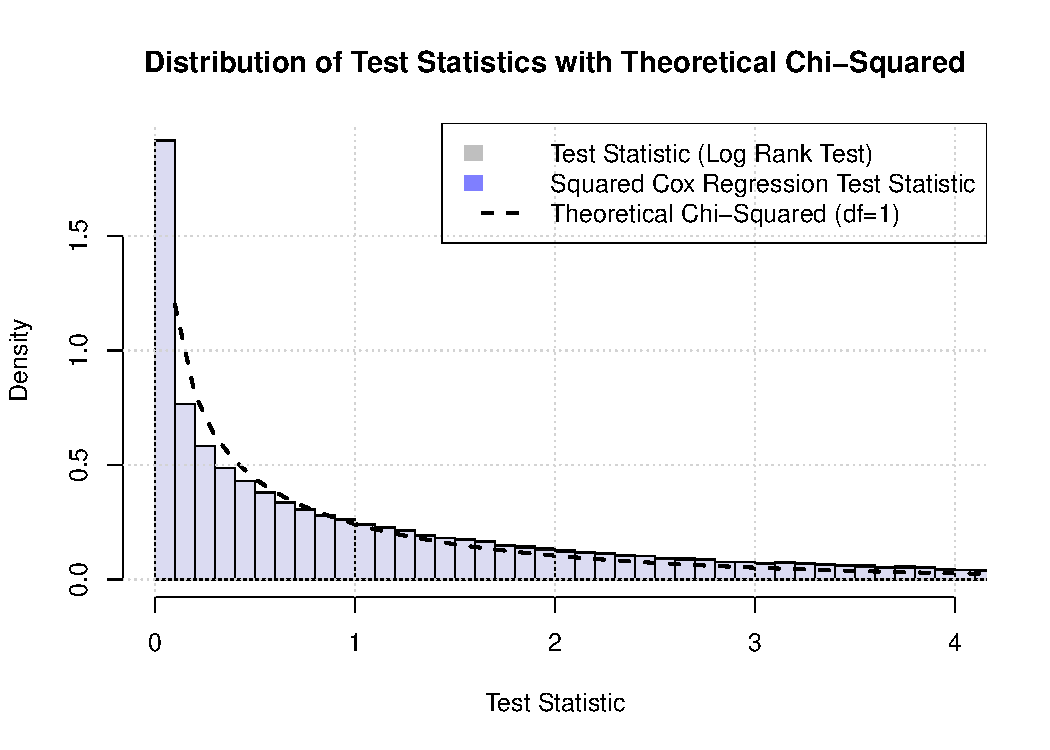
\includegraphics[width=\maxwidth]{figure/chi_squared-1} 

}


\end{knitrout}
    \caption{Distribution of Test Statistics with Theoretical Chi-Squared (\( \chi^2_{(1)} \)). The gray bars represent Log-Rank test statistics, the blue bars represent squared Cox regression test statistics, and the dashed line represents the theoretical \( \chi^2_{(1)} \) distribution.}
    \label{fig:test_statistics}
\end{figure}




\begin{figure}[H]
    \centering
\begin{knitrout}
\definecolor{shadecolor}{rgb}{0.969, 0.969, 0.969}\color{fgcolor}

{\centering 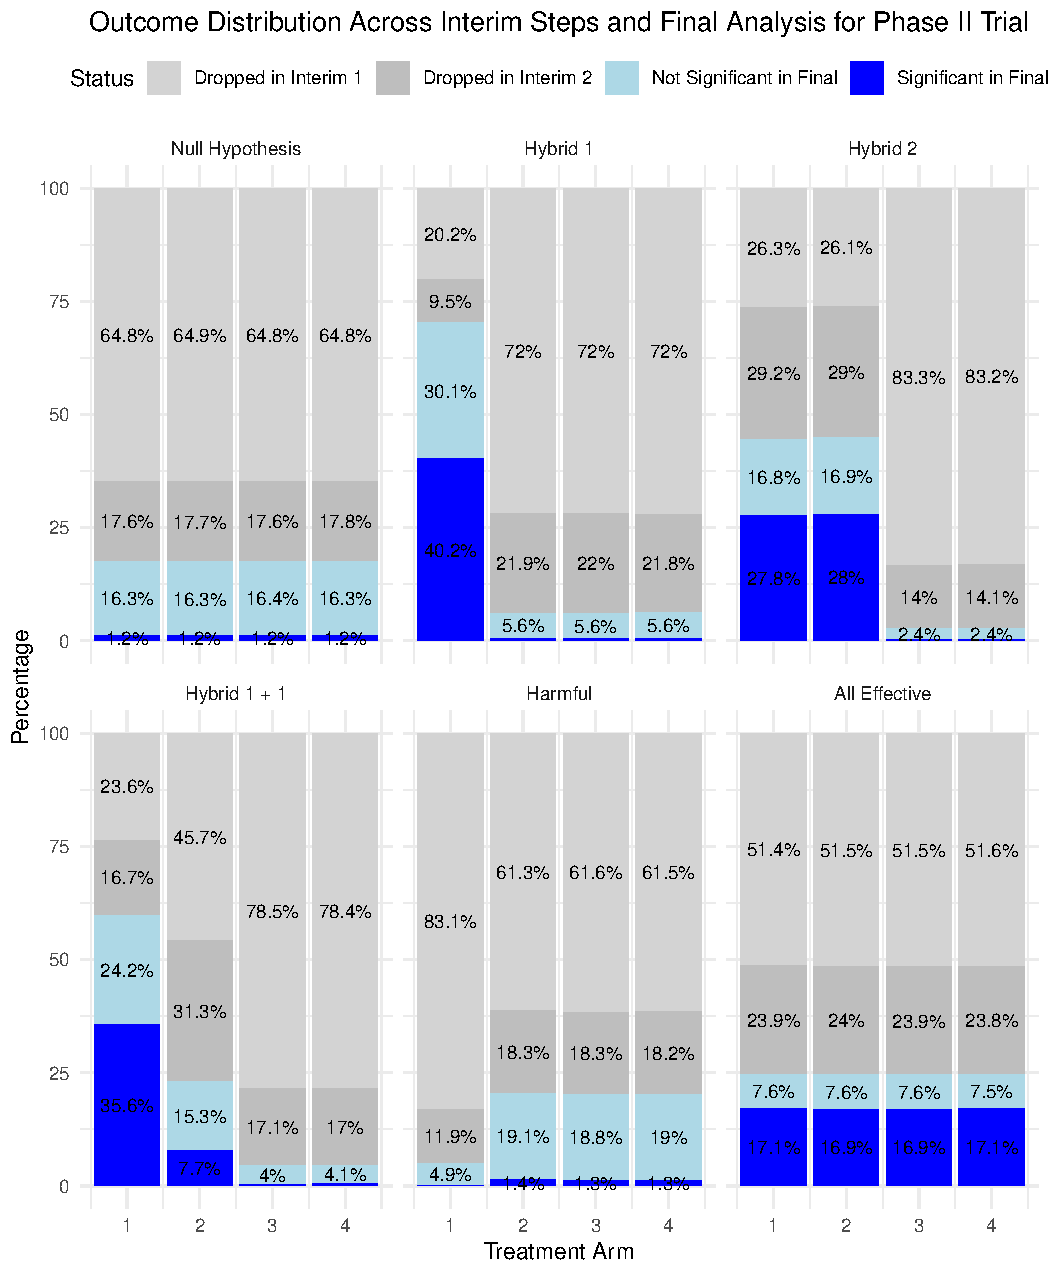
\includegraphics[width=\maxwidth]{figure/barplots_phase2-1} 

}


\end{knitrout}
    \caption{Outcome distribution across interim steps and final analysis for different scenarios for Phase II Trial. In the visualization, percentages below 1\% are omitted to improve clarity and avoid overcrowding, as such small values can make the chart difficult to interpret. However, for the Null Hypothesis, all percentages are displayed regardless of their size to ensure full visibility. Additionally, all results, including those below 1\%, are fully available in Table \ref{tab:outcome_distribution_phase2} for detailed examination.
}
    \label{fig:outcome_distribution_phase2}
\end{figure}


\begin{landscape}
\label{tab:outcome_distribution_phase2}
% latex table generated in R 4.4.1 by xtable 1.8-4 package
% Sun Dec  8 20:02:38 2024
\begin{table}[ht]
\centering
\begin{tabular}{rrllll}
  \hline
Scenario & TreatmentArm & Dropped in Interim 1 & Dropped in Interim 2 & Not Significant in Final & Significant in Final \\ 
  \hline
  1 &   1 & 129691 (64.85\%) & 35252 (17.63\%) & 16.32\% (16.25\% ; 16.39\%) & 1.21\% (1.19\% ; 1.23\%) \\ 
    1 &   2 & 129707 (64.85\%) & 35418 (17.71\%) & 16.28\% (16.21\% ; 16.36\%) & 1.15\% (1.13\% ; 1.17\%) \\ 
    1 &   3 & 129698 (64.85\%) & 35189 (17.59\%) & 16.38\% (16.31\% ; 16.45\%) & 1.17\% (1.15\% ; 1.2\%) \\ 
    1 &   4 & 129569 (64.78\%) & 35544 (17.77\%) & 16.27\% (16.2\% ; 16.34\%) & 1.17\% (1.15\% ; 1.2\%) \\ 
   \hline 
  2 &   1 & 40470 (20.24\%) & 18931 (9.47\%) & 30.08\% (29.99\% ; 30.17\%) & 40.22\% (40.12\% ; 40.31\%) \\ 
    2 &   2 & 143911 (71.96\%) & 43768 (21.88\%) & 5.61\% (5.56\% ; 5.65\%) & 0.56\% (0.54\% ; 0.57\%) \\ 
    2 &   3 & 143903 (71.95\%) & 43906 (21.95\%) & 5.56\% (5.52\% ; 5.61\%) & 0.53\% (0.52\% ; 0.55\%) \\ 
    2 &   4 & 143947 (71.97\%) & 43571 (21.79\%) & 5.65\% (5.6\% ; 5.69\%) & 0.59\% (0.58\% ; 0.61\%) \\ 
   \hline 
  3 &   1 & 52528 (26.26\%) & 58327 (29.16\%) & 16.8\% (16.72\% ; 16.87\%) & 27.77\% (27.69\% ; 27.86\%) \\ 
    3 &   2 & 52278 (26.14\%) & 57911 (28.96\%) & 16.88\% (16.81\% ; 16.96\%) & 28.02\% (27.93\% ; 28.11\%) \\ 
    3 &   3 & 166530 (83.26\%) & 27971 (13.99\%) & 2.43\% (2.4\% ; 2.46\%) & 0.32\% (0.31\% ; 0.33\%) \\ 
    3 &   4 & 166384 (83.19\%) & 28248 (14.12\%) & 2.39\% (2.36\% ; 2.42\%) & 0.29\% (0.28\% ; 0.3\%) \\ 
   \hline 
  4 &   1 & 47148 (23.57\%) & 33310 (16.66\%) & 24.19\% (24.1\% ; 24.27\%) & 35.58\% (35.49\% ; 35.68\%) \\ 
    4 &   2 & 91379 (45.69\%) & 62640 (31.32\%) & 15.26\% (15.19\% ; 15.33\%) & 7.73\% (7.68\% ; 7.79\%) \\ 
    4 &   3 & 156959 (78.48\%) & 34153 (17.08\%) & 4.03\% (3.99\% ; 4.06\%) & 0.42\% (0.41\% ; 0.43\%) \\ 
    4 &   4 & 156825 (78.41\%) & 34095 (17.05\%) & 4.08\% (4.05\% ; 4.12\%) & 0.46\% (0.44\% ; 0.47\%) \\ 
   \hline 
  5 &   1 & 166235 (83.12\%) & 23839 (11.92\%) & 4.89\% (4.85\% ; 4.93\%) & 0.07\% (0.07\% ; 0.08\%) \\ 
    5 &   2 & 122629 (61.31\%) & 36504 (18.25\%) & 19.05\% (18.98\% ; 19.13\%) & 1.38\% (1.36\% ; 1.4\%) \\ 
    5 &   3 & 123135 (61.57\%) & 36605 (18.3\%) & 18.84\% (18.76\% ; 18.91\%) & 1.29\% (1.27\% ; 1.32\%) \\ 
    5 &   4 & 122927 (61.46\%) & 36458 (18.23\%) & 19.04\% (18.96\% ; 19.12\%) & 1.27\% (1.25\% ; 1.29\%) \\ 
   \hline 
  6 &   1 & 102786 (51.39\%) & 47810 (23.91\%) & 7.64\% (7.59\% ; 7.69\%) & 17.06\% (16.99\% ; 17.13\%) \\ 
    6 &   2 & 103058 (51.53\%) & 47900 (23.95\%) & 7.6\% (7.54\% ; 7.65\%) & 16.93\% (16.85\% ; 17\%) \\ 
    6 &   3 & 103088 (51.54\%) & 47849 (23.92\%) & 7.59\% (7.54\% ; 7.64\%) & 16.94\% (16.87\% ; 17.02\%) \\ 
    6 &   4 & 103227 (51.61\%) & 47549 (23.77\%) & 7.53\% (7.47\% ; 7.58\%) & 17.09\% (17.01\% ; 17.16\%) \\ 
   \hline 
 \hline
\end{tabular}
\caption{Outcome Distribution Across Interim Steps and Final Analysis in Phase II Trial (with 95\% Confidence Intervals for the Final Analysis). Note: The maximum Monte Carlo Standard Error is calculated on the following page (Equation~\ref{eq:mcse}).} 
\label{tab:outcome_distribution}
\end{table}

\end{landscape}

\begin{equation}
\text{MCSE} = \frac{s}{\sqrt{n}} = \frac{\sqrt{\hat{p}(1 - \hat{p})}}{\sqrt{n}} = \frac{\sqrt{0.51393 \times 0.48607}}{\sqrt{200000}} = 0.00112 \label{eq:mcse}
\end{equation}

The maximal Monte Carlo standard error (MCSE) for Phase III is 0.00112.


\paragraph{Ethical Considerations}

The "Drop-the-Losers" design is highly aligned with ethical principles in clinical trials, as it minimizes patient exposure to suboptimal or harmful therapies. By incorporating interim analyses to identify and eliminate ineffective or harmful treatment arms, the design ensures that only effective treatments progress to later stages. This approach reduces the risk of advancing ineffective treatments, which could otherwise expose patients to unnecessary risks and compromise the trial's efficiency.

To further evaluate the risk of ineffective arms advancing, we calculated the probability of at least one ineffective treatment arm progressing at each stage based on the simulation results. Table~\ref{tab:ineffective_arm_probability_interim2} presents these probabilities for Interim Analysis 2, while Table~\ref{tab:ineffective_arm_probability_final} provides the corresponding probabilities for the final analysis. These calculations demonstrate the robustness of the statistical thresholds and decision-making mechanisms, ensuring that ineffective treatments are identified and removed with high probability.

For example, in Scenario 1 (Null Hypothesis), where all arms are ineffective, the probability of an ineffective arm advancing to Interim 2 was 1.000, as expected. In hybrid scenarios, such as "Hybrid 1" and "Hybrid 2," where a mix of effective and ineffective arms is present, the probabilities of advancing ineffective arms were lower but non-negligible, reflecting the inherent trade-offs in adaptive trial designs. By contrast, in the "All Effective" scenario, the design effectively ensured that all promising arms progressed without advancing any ineffective treatments.



\begin{table}[ht]
    \centering
    \caption{Probability of Ineffective Arms Advancing to Interim Analysis 2 Across Scenarios}
    \label{tab:ineffective_arm_probability_interim2}
    \begin{tabular}{ccccc}
        \toprule
        \textbf{Scenario} & \textbf{Number of Arms} & \textbf{Total Number of Arms} & \textbf{Probability} & \textbf{MCSE} \\
        \midrule
        1 & 161323 & 161323 & 1.000 & 0.000 \\
        2 & 135615 & 184527 & 0.735 & 0.0012 \\
        3 & 28843  & 192748 & 0.150 & 0.0021 \\
        4 & 69695  & 188636 & 0.369 & 0.0018 \\
        5 & 154851 & 154851 & 1.000 & 0.000 \\
        6 & 0      & 197740 & 0.000 & 0.000 \\
        \bottomrule
    \end{tabular}
\end{table}



\begin{table}[ht]
    \centering
    \caption{Probability of Ineffective Arms Advancing to Final Analysis Across Scenarios}
    \label{tab:ineffective_arm_probability_final}
    \begin{tabular}{ccccc}
        \toprule
        \textbf{Scenario} & \textbf{Number of Arms} & \textbf{Total Number of Arms} & \textbf{Probability} & \textbf{MCSE} \\
        \midrule
        1 & 111868 & 111868 & 1.000 & 0.000 \\
        2 & 31809  & 140728 & 0.226 & 0.0011 \\
        3 & 4851   & 168442 & 0.029 & 0.0004 \\
        4 & 16003  & 156922 & 0.102 & 0.0008 \\
        5 & 100750 & 100750 & 1.000 & 0.000 \\
        6 & 0      & 189798 & 0.000 & 0.000 \\
        \bottomrule
    \end{tabular}
\end{table}



\subsection{Results: Phase III Trial} \label{sec:simulation_results_phase3}

The Phase III trial simulations yielded results that were consistent with those observed in the Phase II study. Given that the underlying assumptions and methods used in Phase III largely mirrored those of Phase II, the numerical findings did not exhibit significant deviations. Consequently, this section focuses on summarizing the key observations without delving into exhaustive details.

The Type I and Type II error rates in the Phase III simulations were well-controlled and aligned closely with the expectations set by Phase II results. Specifically, the Type I error rate remained robustly controlled below the nominal 2.5\% threshold, reflecting the design's capacity to minimize false positives. Similarly, the power to detect true effects, even under complex scenarios such as "Hybrid 1" and "Hybrid 2," was comparable to that achieved in Phase II, demonstrating the scalability of the "Drop-the-Losers" design across trial phases.

\begin{figure}[H]
    \centering
\begin{knitrout}
\definecolor{shadecolor}{rgb}{0.969, 0.969, 0.969}\color{fgcolor}

{\centering 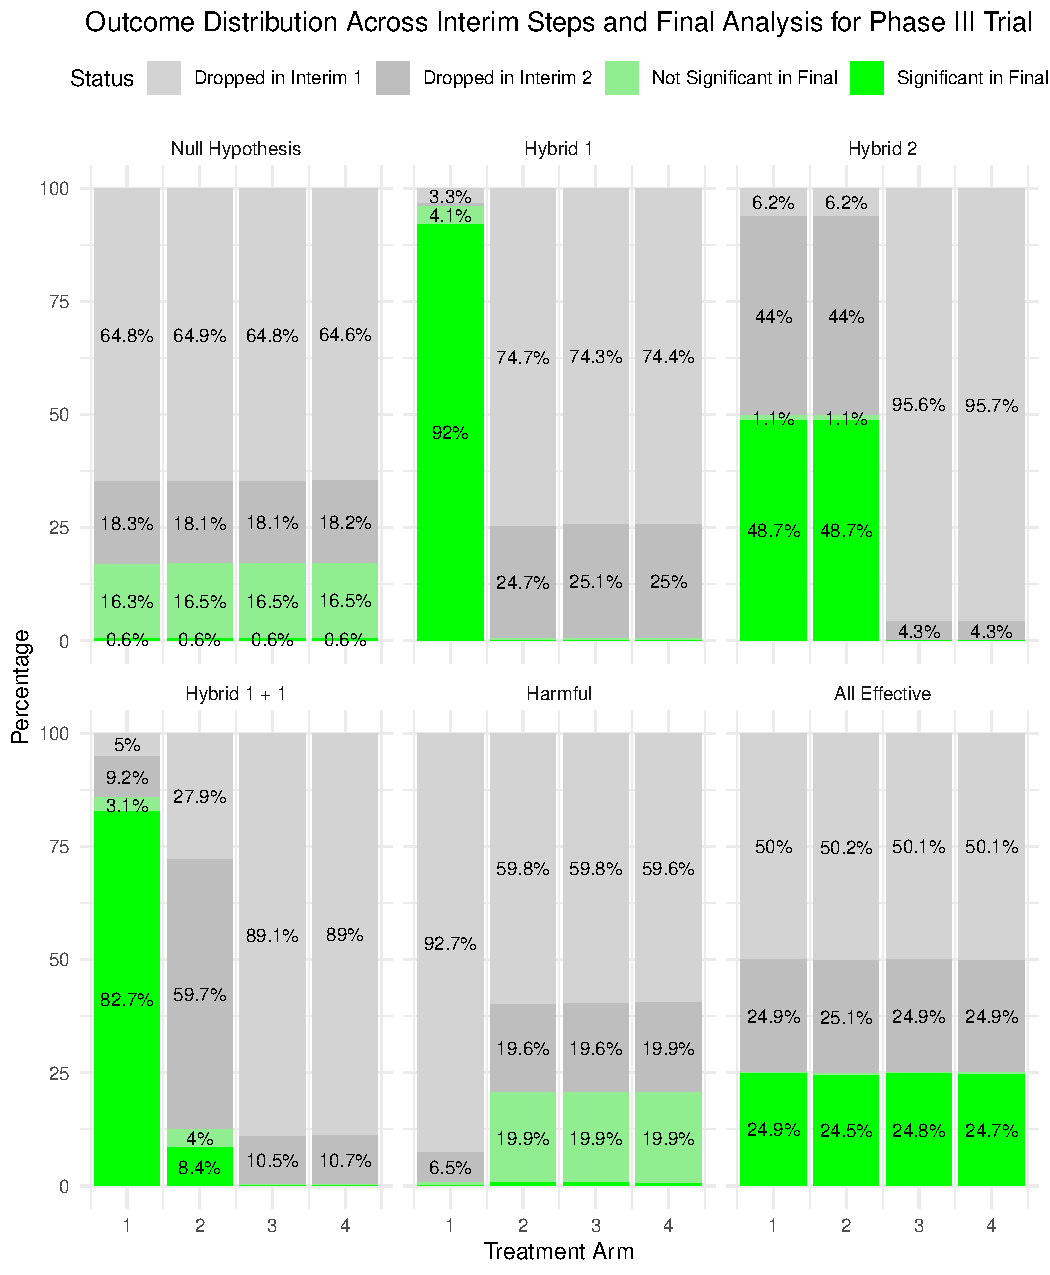
\includegraphics[width=\maxwidth]{figure/barplots_phase3-1} 

}


\end{knitrout}
    \caption{Outcome distribution across interim steps and final analysis for different scenarios for Phase III Trial. In the visualization, percentages below 1\% are omitted to improve clarity and avoid overcrowding, as such small values can make the chart difficult to interpret. However, for the Null Hypothesis, all percentages are displayed regardless of their size to ensure full visibility. Additionally, all results, including those below 1\%, are fully available in Table~\ref{tab:outcome_distribution_phase3} for detailed examination.
}
    \label{fig:outcome_distribution_phase3}
\end{figure}






\begin{landscape}
\label{tab:outcome_distribution_phase3}
% latex table generated in R 4.4.1 by xtable 1.8-4 package
% Sun Dec  8 20:03:10 2024
\begin{table}[ht]
\centering
\begin{tabular}{rrllll}
  \hline
Scenario & TreatmentArm & Dropped in Interim 1 & Dropped in Interim 2 & Not Significant in Final & Significant in Final \\ 
  \hline
  1 &   1 & 129578 (64.79\%) & 36540 (18.27\%) & 16.34\% (16.27\% ; 16.41\%) & 0.6\% (0.59\% ; 0.62\%) \\ 
    1 &   2 & 129710 (64.85\%) & 36203 (18.1\%) & 16.46\% (16.39\% ; 16.53\%) & 0.58\% (0.57\% ; 0.6\%) \\ 
    1 &   3 & 129643 (64.82\%) & 36233 (18.12\%) & 16.49\% (16.41\% ; 16.56\%) & 0.58\% (0.56\% ; 0.59\%) \\ 
    1 &   4 & 129285 (64.64\%) & 36407 (18.2\%) & 16.55\% (16.47\% ; 16.62\%) & 0.61\% (0.59\% ; 0.62\%) \\ 
   \hline 
  2 &   1 & 6699 (3.35\%) & 1168 (0.58\%) & 4.06\% (4.02\% ; 4.1\%) & 92.01\% (91.96\% ; 92.06\%) \\ 
    2 &   2 & 149396 (74.7\%) & 49393 (24.7\%) & 0.57\% (0.55\% ; 0.58\%) & 0.04\% (0.04\% ; 0.04\%) \\ 
    2 &   3 & 148529 (74.26\%) & 50227 (25.11\%) & 0.59\% (0.57\% ; 0.6\%) & 0.04\% (0.03\% ; 0.04\%) \\ 
    2 &   4 & 148713 (74.36\%) & 50031 (25.02\%) & 0.59\% (0.57\% ; 0.6\%) & 0.04\% (0.04\% ; 0.05\%) \\ 
   \hline 
  3 &   1 & 12495 (6.25\%) & 87928 (43.96\%) & 1.05\% (1.03\% ; 1.07\%) & 48.74\% (48.64\% ; 48.83\%) \\ 
    3 &   2 & 12495 (6.25\%) & 88029 (44.01\%) & 1.06\% (1.04\% ; 1.08\%) & 48.68\% (48.58\% ; 48.78\%) \\ 
    3 &   3 & 191252 (95.63\%) & 8632 (4.32\%) & 0.05\% (0.05\% ; 0.05\%) & 0.01\% (0.01\% ; 0.01\%) \\ 
    3 &   4 & 191331 (95.67\%) & 8529 (4.26\%) & 0.06\% (0.06\% ; 0.07\%) & 0.01\% (0.01\% ; 0.01\%) \\ 
   \hline 
  4 &   1 & 10006 (5\%) & 18455 (9.23\%) & 3.12\% (3.08\% ; 3.15\%) & 82.65\% (82.58\% ; 82.73\%) \\ 
    4 &   2 & 55759 (27.88\%) & 119349 (59.67\%) & 4.01\% (3.97\% ; 4.04\%) & 8.44\% (8.39\% ; 8.49\%) \\ 
    4 &   3 & 178265 (89.13\%) & 21085 (10.54\%) & 0.29\% (0.28\% ; 0.3\%) & 0.03\% (0.03\% ; 0.04\%) \\ 
    4 &   4 & 177913 (88.96\%) & 21458 (10.73\%) & 0.29\% (0.28\% ; 0.3\%) & 0.02\% (0.02\% ; 0.02\%) \\ 
   \hline 
  5 &   1 & 185311 (92.66\%) & 12971 (6.49\%) & 0.86\% (0.84\% ; 0.88\%) & 0\% (0\% ; 0\%) \\ 
    5 &   2 & 119619 (59.81\%) & 39217 (19.61\%) & 19.91\% (19.83\% ; 19.99\%) & 0.67\% (0.66\% ; 0.69\%) \\ 
    5 &   3 & 119550 (59.77\%) & 39291 (19.65\%) & 19.93\% (19.85\% ; 20.01\%) & 0.65\% (0.64\% ; 0.67\%) \\ 
    5 &   4 & 119137 (59.57\%) & 39716 (19.86\%) & 19.94\% (19.86\% ; 20.01\%) & 0.64\% (0.62\% ; 0.65\%) \\ 
   \hline 
  6 &   1 & 99928 (49.96\%) & 49800 (24.9\%) & 0.28\% (0.27\% ; 0.29\%) & 24.86\% (24.77\% ; 24.94\%) \\ 
    6 &   2 & 100374 (50.19\%) & 50109 (25.05\%) & 0.26\% (0.25\% ; 0.27\%) & 24.5\% (24.41\% ; 24.58\%) \\ 
    6 &   3 & 100116 (50.06\%) & 49775 (24.89\%) & 0.28\% (0.27\% ; 0.29\%) & 24.77\% (24.69\% ; 24.86\%) \\ 
    6 &   4 & 100187 (50.09\%) & 49784 (24.89\%) & 0.29\% (0.28\% ; 0.31\%) & 24.72\% (24.64\% ; 24.8\%) \\ 
   \hline 
 \hline
\end{tabular}
\caption{Outcome Distribution Across Interim Steps and Final Analysis in Phase III Trial (with 95\% Confidence Intervals for the Final Analysis). Note: The maximum Monte Carlo Standard Error is calculated on the following page (Equation~\ref{eq:mcse2}).} 
\label{tab:outcome_distribution}
\end{table}

\end{landscape}

\begin{equation}
\text{MCSE} = \frac{s}{\sqrt{n}} = \frac{\sqrt{\hat{p}(1 - \hat{p})}}{\sqrt{n}} = \frac{\sqrt{0.49964 \times 0.50036}}{\sqrt{200000}} = 0.00112 \label{eq:mcse1}
\end{equation}

The maximal Monte Carlo standard error (MCSE) is 0.00112



\newpage
\section{Discussion} \label{sec:discussion}

This study presents a significant advancement in the methodological framework of adaptive clinical trial designs by extending the "Drop-the-Losers" approach to accommodate binary and survival endpoints. This extension fills a critical gap in existing methodologies, enhancing the design's applicability to Phase II/III oncology trials, where treatment selection is essential for optimizing patient outcomes and expediting drug development. The proposed modifications align with recommended clinical endpoints, allowing trials to incorporate real-world complexities without compromising statistical rigor.

The primary contributions of this work lie in the extension to other endpoint types. By addressing binary and survival endpoints, the methodology expands beyond Wason's original framework, which was limited to continuous endpoints.

Despite these advancements, the proposed design faces several limitations. One major challenge is the reliance on normal approximations, which may not fully capture the statistical properties of binary and survival endpoints. This could lead to potential biases in treatment selection, particularly under scenarios where endpoint distributions deviate from normality. Another limitation is the maturity of long-term survival endpoints, which may not be fully realized during early interim analyses. A potential solution involves dynamically updating endpoints throughout the trial, such as starting with objective response rate (ORR) at the first analysis, transitioning to progression-free survival (PFS) at the second, and concluding with overall survival (OS) at the final stage. However, this approach introduces additional complexity, requiring careful handling of correlations between surrogate and final endpoints.

Generalizability is another consideration. While the design demonstrates robust performance in oncology trials, its direct applicability to other therapeutic areas remains uncertain. Variability in endpoint dynamics, sample size requirements, and trial objectives across disciplines may necessitate further adaptation. For instance, non-oncology trials might involve endpoints with fundamentally different statistical properties or clinical implications, which could affect the performance of the "Drop-the-Losers" approach.

In terms of ethical considerations, the "Drop-the-Losers" design minimizes patient exposure to suboptimal or harmful treatments by eliminating less effective arms at interim stages. This aligns with the ethical principle of beneficence, ensuring that trial participants receive treatments with the highest likelihood of benefit. For example, in the simulation scenarios, the design consistently identified and removed ineffective or harmful arms early in the trial, reducing unnecessary risk and resource expenditure.


In conclusion, this study represents a substantial step forward in clinical trial methodologies. By addressing key limitations of previous designs and extending their applicability to binary and survival endpoints, the "Drop-the-Losers" approach offers a powerful tool for Phase II/III oncology trials and beyond. While further validation and refinement are needed to address specific limitations, the proposed framework provides a strong foundation for more efficient, ethical, and scientifically robust clinical trials. Future work could explore extensions to other therapeutic areas, refine statistical assumptions, and incorporate additional endpoints to further enhance the versatility and impact of this design.


% References and appendices
% =============================================================================

\pagebreak

\appendix
\section*{Appendix} \label{sec:app}
\addcontentsline{toc}{section}{Appendix}
\renewcommand{\thesection}{\Alph{section}}

\section{Covariance between test statistics based on continuous endpoints} \label{sec:app_derivations}

We first define the standardized difference between the two groups for a continuous outcome:

\begin{align*}
Z_j^{(k)} = \left(\frac{1}{n_j} \sum_{i=1}^{n_j} X_{ki} - \frac{1}{n_j} \sum_{i=1}^{n_j} X_{0i}\right) \sqrt{\frac{n_j}{2\sigma^2}}
\end{align*}

Assume that \( p > j \), \( n_p > n_j \), and we are looking at \({k = m}\). We want to compute the following covariance:

\[
\text{Cov}\left(Z_j^{(k)}; Z_p^{(m)}\right)
\]

The covariance between the two standardized variables is given by:

\begin{align*}
\text{Cov}\left(Z_j^{(k)}; Z_p^{(m)}\right)
& = \text{Cov}\left( \left( \frac{1}{n_j} \sum_{i=1}^{n_j} X_{ki} - \frac{1}{n_j} \sum_{i=1}^{n_j} X_{0i} \right) \sqrt{\frac{n_j}{2\sigma^2}}; \right. \\
& \quad \left. \left( \frac{1}{n_p} \sum_{i=1}^{n_p} X_{ki} - \frac{1}{n_p} \sum_{i=1}^{n_p} X_{0i} \right) \sqrt{\frac{n_p}{2\sigma^2}} \right) \\
& = \frac{\sqrt{n_j n_p}}{2 \sigma^2} \cdot \text{Cov}\left( \frac{1}{n_j} \sum_{i=1}^{n_j} X_{ki} - \frac{1}{n_j} \sum_{i=1}^{n_j} X_{0i}; \frac{1}{n_p} \sum_{i=1}^{n_p} X_{ki} - \frac{1}{n_p} \sum_{i=1}^{n_p} X_{0i} \right)
\end{align*}

By splitting the covariance terms, we get:

\begin{align*}
\text{Cov}\left(Z_j^{(k)}; Z_p^{(m)}\right)
& = \frac{\sqrt{n_j n_p}}{2 \sigma^2} \left[ \text{Cov}\left( \frac{1}{n_j} \sum_{i=1}^{n_j} X_{ki}; \frac{1}{n_p} \sum_{i=1}^{n_p} X_{ki} \right) \right. \\
& \quad - \text{Cov}\left( \frac{1}{n_j} \sum_{i=1}^{n_j} X_{ki}; \frac{1}{n_p} \sum_{i=1}^{n_p} X_{0i} \right) \\
& \quad - \text{Cov}\left( \frac{1}{n_j} \sum_{i=1}^{n_j} X_{0i}; \frac{1}{n_p} \sum_{i=1}^{n_p} X_{ki} \right) \\
& \quad \left. + \text{Cov}\left( \frac{1}{n_j} \sum_{i=1}^{n_j} X_{0i}; \frac{1}{n_p} \sum_{i=1}^{n_p} X_{0i} \right) \right]
\end{align*}

The computation of each covariance term leads to:

\begin{align*}
\text{Cov}\left(Z_j^{(k)}; Z_p^{(m)}\right)
& = \frac{\sqrt{n_j n_p}}{2 \sigma^2} \left[ \frac{1}{n_j n_p} \sum_{i=1}^{n_j} \text{Cov}\left( X_{ki}, X_{ki} \right) + \frac{1}{n_j n_p} \sum_{i=1}^{n_j} \text{Cov}\left( X_{0i}, X_{0i} \right) \right] \\
& = \frac{\sqrt{n_j n_p}}{2 \sigma^2} \left[ \frac{1}{n_j n_p} \cdot 2n_j \sigma^2 \right] \\
& = \sqrt{\frac{n_j}{n_p}}
\end{align*}


Assume that \( p > j \), \( n_p > n_j \), and we are considering \({k \neq m}\). We want to compute the following covariance:

\[
\text{Cov}\left(Z_j^{(k)}; Z_p^{(m)}\right)
\]

The covariance between the two standardized variables is given by:

\begin{align*}
\text{Cov}\left(Z_j^{(k)}; Z_p^{(m)}\right)
& = \text{Cov}\left( \left( \frac{1}{n_j} \sum_{i=1}^{n_j} X_{ki} - \frac{1}{n_j} \sum_{i=1}^{n_j} X_{0i} \right) \sqrt{\frac{n_j}{2\sigma^2}}; \right. \\
& \quad \left. \left( \frac{1}{n_p} \sum_{i=1}^{n_p} X_{mi} - \frac{1}{n_p} \sum_{i=1}^{n_p} X_{0i} \right) \sqrt{\frac{n_p}{2\sigma^2}} \right)
\end{align*}

Next, we break down the covariance term:

\begin{align*}
\text{Cov}\left(Z_j^{(k)}; Z_p^{(m)}\right)
& = \frac{\sqrt{n_j n_p}}{2 \sigma^2} \cdot \text{Cov}\left( \frac{1}{n_j} \sum_{i=1}^{n_j} X_{ki} - \frac{1}{n_j} \sum_{i=1}^{n_j} X_{0i}; \frac{1}{n_p} \sum_{i=1}^{n_p} X_{mi} - \frac{1}{n_p} \sum_{i=1}^{n_p} X_{0i} \right)
\end{align*}

Expanding the covariance terms results in:

\begin{align*}
\text{Cov}\left(Z_j^{(k)}; Z_p^{(m)}\right)
& = \frac{\sqrt{n_j n_p}}{2 \sigma^2} \left[ \text{Cov}\left( \frac{1}{n_j} \sum_{i=1}^{n_j} X_{ki}; \frac{1}{n_p} \sum_{i=1}^{n_p} X_{mi} \right) \right. \\
& \quad - \text{Cov}\left( \frac{1}{n_j} \sum_{i=1}^{n_j} X_{ki}; \frac{1}{n_p} \sum_{i=1}^{n_p} X_{0i} \right) \\
& \quad - \text{Cov}\left( \frac{1}{n_j} \sum_{i=1}^{n_j} X_{0i}; \frac{1}{n_p} \sum_{i=1}^{n_p} X_{mi} \right) \\
& \quad \left. + \text{Cov}\left( \frac{1}{n_j} \sum_{i=1}^{n_j} X_{0i}; \frac{1}{n_p} \sum_{i=1}^{n_p} X_{0i} \right) \right]
\end{align*}

Simplifying further:

\begin{align*}
\text{Cov}\left(Z_j^{(k)}; Z_p^{(m)}\right)
& = \frac{\sqrt{n_j n_p}}{2\sigma^2} \left[ \text{Cov}\left( \frac{1}{n_j} \sum_{i=1}^{n_j} X_{ki}; \frac{1}{n_p} \sum_{i=1}^{n_p} X_{mi} \right) \right. \\
& \quad \left. + \text{Cov}\left( \frac{1}{n_j} \sum_{i=1}^{n_j} X_{0i}; \frac{1}{n_p} \sum_{i=1}^{n_p} X_{0i} \right) \right]
\end{align*}

Finally, we evaluate the covariance terms:

\begin{align*}
\text{Cov}\left(Z_j^{(k)}; Z_p^{(m)}\right)
& = \frac{\sqrt{n_j n_p}}{2 \sigma^2} \left[ \frac{1}{n_j n_p} \sum_{i=1}^{n_j} \text{Cov}\left(X_{ki}, X_{mi}\right) + \frac{1}{n_j n_p} \sum_{i=1}^{n_j} \text{Cov}\left(X_{0i}, X_{0i}\right) \right] \\
& = \frac{\sqrt{n_j n_p}}{2 \sigma^2} \left[ \frac{1}{n_j n_p} \cdot 0 + \frac{1}{n_j n_p} \cdot n_j \sigma^2 \right] \\
& = \frac{\sqrt{n_j n_p}}{2 \sigma^2} \cdot \frac{\sigma^2}{n_p} \\
& = \frac{1}{2} \cdot \sqrt{\frac{n_j}{n_p}}
\end{align*}



\section{Covariance between test statistics based on binary endpoints} \label{sec:app_derivations_binary}

First, we consider the case where \( k = m \), and assume that the probability \( p \) is constant. We aim to compute the covariance between \( Z_j^{(k)} \) and \( Z_p^{(m)} \).

\begin{align*}
\text{Cov}(Z_j^{(k)}, Z_p^{(m)})
&= \text{Cov}\left(\frac{1}{n_j} \sum_{i=1}^{n_j} (X_{ki} - X_{0i}), \frac{1}{n_p} \sum_{i=1}^{n_p} (X_{ki} - X_{0i})\right) \sqrt{\frac{n_j n_p}{2p(1-p)}} \\
&= \sqrt{\frac{n_j n_p}{2p(1-p)}} \left( \frac{1}{n_j n_p} \sum_{i=1}^{n_j} \text{Cov}(X_{ki}, X_{ki}) - \frac{1}{n_j n_p} \sum_{i=1}^{n_j} \text{Cov}(X_{ki}, X_{0i}) \right)
\end{align*}

Next, simplifying the covariance expression:

\begin{align*}
\text{Cov}(Z_j^{(k)}, Z_p^{(m)})
&= \sqrt{\frac{n_j n_p}{2p(1-p)}} \left( \frac{p(1-p)}{n_j n_p} \right) \\
\end{align*}


Now, we consider the case where \({k \neq m\), and again assume that the probability \( p \) is constant. The covariance between \( Z_j^{(k)} \) and \( Z_p^{(m)} \) can be expanded as follows:

\begin{align*}
\text{Cov}(Z_j^{(k)}, Z_p^{(m)})
&= \text{Cov}\left(\frac{1}{n_j} \sum_{i=1}^{n_j} (X_{ki} - X_{0i}), \frac{1}{n_p} \sum_{i=1}^{n_p} (X_{mi} - X_{0i})\right) \sqrt{\frac{n_j n_p}{2p(1-p)}}
\end{align*}

We first expand the covariance expression:

\begin{align*}
\text{Cov}(Z_j^{(k)}, Z_p^{(m)})
&= \sqrt{\frac{n_j n_p}{2p(1-p)}} \cdot \text{Cov}\left(\frac{1}{n_j} \sum_{i=1}^{n_j} (X_{ki} - X_{0i}), \frac{1}{n_p} \sum_{i=1}^{n_p} (X_{mi} - X_{0i})\right) \\
&= \sqrt{\frac{n_j n_p}{2p(1-p)}} \left[ \text{Cov}\left( \frac{1}{n_j} \sum_{i=1}^{n_j} X_{ki}, \frac{1}{n_p} \sum_{i=1}^{n_p} X_{mi} \right) \right. \\
& \quad \left. - \text{Cov}\left( \frac{1}{n_j} \sum_{i=1}^{n_j} X_{ki}, \frac{1}{n_p} \sum_{i=1}^{n_p} X_{0i} \right) \right. \\
& \quad \left. - \text{Cov}\left( \frac{1}{n_j} \sum_{i=1}^{n_j} X_{0i}, \frac{1}{n_p} \sum_{i=1}^{n_p} X_{mi} \right) \right. \\
& \quad \left. + \text{Cov}\left( \frac{1}{n_j} \sum_{i=1}^{n_j} X_{0i}, \frac{1}{n_p} \sum_{i=1}^{n_p} X_{0i} \right) \right]
\end{align*}

When \( k \neq m \), the random variables \( X_{ki} \) and \( X_{mi} \) are independent. Therefore, the covariance \( \text{Cov}(X_{ki}, X_{mi}) \) is zero, and the corresponding terms vanish:

\begin{align*}
\text{Cov}\left( \frac{1}{n_j} \sum_{i=1}^{n_j} X_{ki}, \frac{1}{n_p} \sum_{i=1}^{n_p} X_{mi} \right) &= 0
\end{align*}

This leaves us with the remaining covariance terms:

\begin{align*}
\text{Cov}(Z_j^{(k)}, Z_p^{(m)})
&= \sqrt{\frac{n_j n_p}{2p(1-p)}} \left[ - \text{Cov}\left( \frac{1}{n_j} \sum_{i=1}^{n_j} X_{ki}, \frac{1}{n_p} \sum_{i=1}^{n_p} X_{0i} \right) \right. \\
& \quad \left. - \text{Cov}\left( \frac{1}{n_j} \sum_{i=1}^{n_j} X_{0i}, \frac{1}{n_p} \sum_{i=1}^{n_p} X_{mi} \right) \right. \\
& \quad \left. + \text{Cov}\left( \frac{1}{n_j} \sum_{i=1}^{n_j} X_{0i}, \frac{1}{n_p} \sum_{i=1}^{n_p} X_{0i} \right) \right]
\end{align*}

The remaining covariance terms involve \( X_{0i} \), which represents the control group. Since the control group is common across both \( j \) and \( p \), we can simplify the covariance of the control group with itself:

\begin{align*}
\text{Cov}\left( \frac{1}{n_j} \sum_{i=1}^{n_j} X_{0i}, \frac{1}{n_p} \sum_{i=1}^{n_p} X_{0i} \right) &= \frac{p(1-p)}{n_j n_p}
\end{align*}

Substituting this result back into the original expression gives us:

\begin{align*}
\text{Cov}(Z_j^{(k)}, Z_p^{(m)})
&= \sqrt{\frac{n_j n_p}{2p(1-p)}} \cdot \frac{p(1-p)}{n_j n_p} \\
&= \frac{1}{2} \cdot \sqrt{\frac{n_j}{n_p}}
\end{align*}

Thus, for \( k \neq m \), the covariance simplifies to:

\[
\text{Cov}(Z_j^{(k)}, Z_p^{(m)}) = \frac{1}{2} \cdot \sqrt{\frac{n_j}{n_p}}
\]


\section{Covariance between test statistics based on survival endpoints} \label{sec:app_derivations_survival}

We start by defining the standardized statistic \( Z_j^{(k)} \), which approximates the log hazard ratio for arm \( k \) in stage \( j \):

\[
Z_j^{(k)} \approx \frac{\log \widehat{HR}_{kj}}{\sqrt{\frac{4}{d_j^{(o)} + d_j^{(k)}}}} = \log \widehat{HR}_{kj} \cdot \sqrt{\frac{d_j^{(o)} + d_j^{(k)}}{4}}
\]

where \( \widehat{HR}_{kj} \) is the hazard ratio estimate for arm \( k \) in stage \( j \), and \( d_j^{(o)} \) and \( d_j^{(k)} \) are the event counts for the control and treatment arms, respectively.

We assume \( k = m \) and further that \( p > j \), meaning that the sample size in stage \( p \) is greater than in stage \( j \) \( (n_p > n_j) \). Now, we aim to compute the covariance between \( Z_j^{(k)} \) and \( Z_p^{(k)} \):

\[
\text{Cov} \left( Z_j^{(k)} , Z_p^{(k)} \right) = \frac{1}{4} \text{Cov}\left( \log \widehat{HR}_{kj} \times \sqrt{d_j^{(o)} + d_j^{(k)}} ; \log \widehat{HR}_{kp} \times \sqrt{d_p^{(o)} + d_p^{(k)}} \right)
\]


Next, we use an approximation for the hazard ratio between studies \( j \) and \( p \):

\[
\widehat{HR}_{kp} \approx \widehat{HR}_{kj}^{\left(\frac{d_j^{(o)} + d_j^{(k)}}{d_p^{(o)} + d_p^{(k)}}\right)} \times \widehat{HR}_{\overline{kj}}^{\left(1 - \frac{d_j^{(o)} + d_j^{(k)}}{d_p^{(o)} + d_p^{(k)}}\right)}
\]

This expresses the hazard ratio in stage \( p \) as a weighted average of the hazard ratio in stage \( j \) and its complement.

Taking the logarithm of the hazard ratio approximation gives:

\[
\log(\widehat{HR}_{kp}) \approx \left(\frac{d_j^{(o)} + d_j^{(k)}}{d_p^{(o)} + d_p^{(k)}}\right) \log(\widehat{HR}_{kj}) + \left(1 - \frac{d_j^{(o)} + d_j^{(k)}}{d_p^{(o)} + d_p^{(k)}}\right) \log(\widehat{HR}_{\overline{kj}})
\]

Now we substitute this back into the covariance expression:

\[
\text{Cov} \left( Z_j^{(k)} , Z_p^{(k)} \right) = \frac{1}{4} \times \text{Cov} \left( \log \widehat{HR}_{kj} , \log \widehat{HR}_{kp} \right) \times \sqrt{(d_j^{(o)} + d_j^{(k)})^3} \times \frac{1}{\sqrt{d_p^{(o)} + d_p^{(k)}}}
\]


Assuming that the hazard ratio estimates across studies are proportional to the event counts, we simplify the covariance term:

\[
\text{Cov} \left( Z_j^{(k)} , Z_p^{(k)} \right) = \frac{1}{4} \times \text{Cov} \left( \log \widehat{HR}_{kj} , \log \widehat{HR}_{kj} \right) \times \frac{(d_j^{(o)} + d_j^{(k)})^{3/2}}{(d_p^{(o)} + d_p^{(k)})^{1/2}}
\]

Given that the covariance of the log hazard ratios is proportional to the event counts, we can further simplify:

\[
\text{Cov} \left( Z_j^{(k)} , Z_p^{(k)} \right) = \frac{1}{4} \times \frac{4 \times (d_j^{(o)} + d_j^{(k)})}{d_j^{(o)} + d_j^{(k)}} \times \sqrt{\frac{d_j^{(o)} + d_j^{(k)}}{d_p^{(o)} + d_p^{(k)}}}
\]

Finally, the covariance simplifies to:

\[
\text{Cov} \left( Z_j^{(k)} , Z_p^{(k)} \right) = \sqrt{\frac{d_j^{(o)} + d_j^{(k)}}{d_p^{(o)} + d_p^{(k)}}}
\]



We now consider the case where \({k \neq m}\) and compute the covariance between \( Z_j^{(k)} \) and \( Z_p^{(m)} \). We start with the same definition for \( Z_j^{(k)} \) and \( Z_p^{(m)} \):

\[
Z_j^{(k)} \approx \log \widehat{HR}_{kj} \cdot \sqrt{\frac{d_j^{(o)} + d_j^{(k)}}{4}}
\]
\[
Z_p^{(m)} \approx \log \widehat{HR}_{mp} \cdot \sqrt{\frac{d_p^{(o)} + d_p^{(m)}}{4}}
\]

where \( \widehat{HR}_{kj} \) and \( \widehat{HR}_{mp} \) are the hazard ratio estimates for arm \( k \) in stage \( j \) and arm \( m \) in stage \( p \), respectively.


Now, we compute the covariance between \( Z_j^{(k)} \) and \( Z_p^{(m)} \):

\[
\text{Cov} \left( Z_j^{(k)} , Z_p^{(m)} \right) = \frac{1}{4} \text{Cov}\left( \log \widehat{HR}_{kj} \cdot \sqrt{d_j^{(o)} + d_j^{(k)}} ; \log \widehat{HR}_{mp} \cdot \sqrt{d_p^{(o)} + d_p^{(m)}} \right)
\]

We expand the covariance term:

\[
\text{Cov} \left( Z_j^{(k)} , Z_p^{(m)} \right) = \frac{1}{4} \cdot \sqrt{(d_j^{(o)} + d_j^{(k)})} \cdot \sqrt{(d_p^{(o)} + d_p^{(m)})} \cdot \text{Cov}\left( \log \widehat{HR}_{kj}, \log \widehat{HR}_{mp} \right)
\]

When \( k \neq m \), the hazard ratio estimates \( \widehat{HR}_{kj} \) and \( \widehat{HR}_{mp} \) are independent, meaning the covariance between \( \log \widehat{HR}_{kj} \) and \( \log \widehat{HR}_{mp} \) is zero:

\[
\text{Cov}\left( \log \widehat{HR}_{kj}, \log \widehat{HR}_{mp} \right) = 0
\]

Thus, the first term involving \( \log \widehat{HR}_{kj} \) and \( \log \widehat{HR}_{mp} \) vanishes, and we are left with the covariance of the control arm terms:

\[
\text{Cov} \left( Z_j^{(k)} , Z_p^{(m)} \right) = \frac{1}{4} \cdot \left( \text{Cov} \left( \log \widehat{HR}_{kj}, \log \widehat{HR}_{\overline{kj}} \right) \right)
\]

This leads to the following simplified covariance expression for the control arm:

\[
\text{Cov} \left( Z_j^{(k)} , Z_p^{(m)} \right) = \frac{1}{4} \times \frac{(d_j^{(o)} + d_j^{(k)})^{3/2}}{(d_p^{(o)} + d_p^{(m)})^{1/2}} \cdot \text{Cov} \left( \log \widehat{HR}_{\overline{kj}}, \log \widehat{HR}_{\overline{mp}} \right)
\]

Given that the hazard ratios \( \widehat{HR}_{\overline{kj}} \) and \( \widehat{HR}_{\overline{mp}} \) are independent for \( k \neq m \), the resulting covariance is proportional to the event counts. Finally, we arrive at:

\[
\text{Cov} \left( Z_j^{(k)} , Z_p^{(m)} \right) = \frac{1}{4} \times \frac{4 \times (d_j^{(o)} + d_j^{(k)})}{d_j^{(o)} + d_j^{(k)}} \times \sqrt{\frac{d_j^{(o)} + d_p^{(m)}}{d_p^{(o)} + d_p^{(m)}}}
\]

The final covariance for \( k \neq m \) is:

\[
\text{Cov} \left( Z_j^{(k)} , Z_p^{(m)} \right) = \frac{1}{2} \cdot \sqrt{\frac{d_j^{(o)} + d_j^{(k)}}{d_p^{(o)} + d_p^{(m)}}}
\]

This result is similar to the case where \( k = m \), but with an additional factor of \( 0.5 \) due to the independence of \( k \) and \( m \).

\section{Additional Simulation Results} \label{sec:app_sim_results}

This appendix provides additional simulation results for a Drop-the-Loser (DLT) design, incorporating both Cox regression and the Log-Rank test. The results are based on \( n = 200'000 \) simulation runs, performed using the function \texttt{simulate\_trial\_log\_rank} for both Phase II and III stages.

\begin{figure}[H]
    \centering
\begin{knitrout}
\definecolor{shadecolor}{rgb}{0.969, 0.969, 0.969}\color{fgcolor}

{\centering 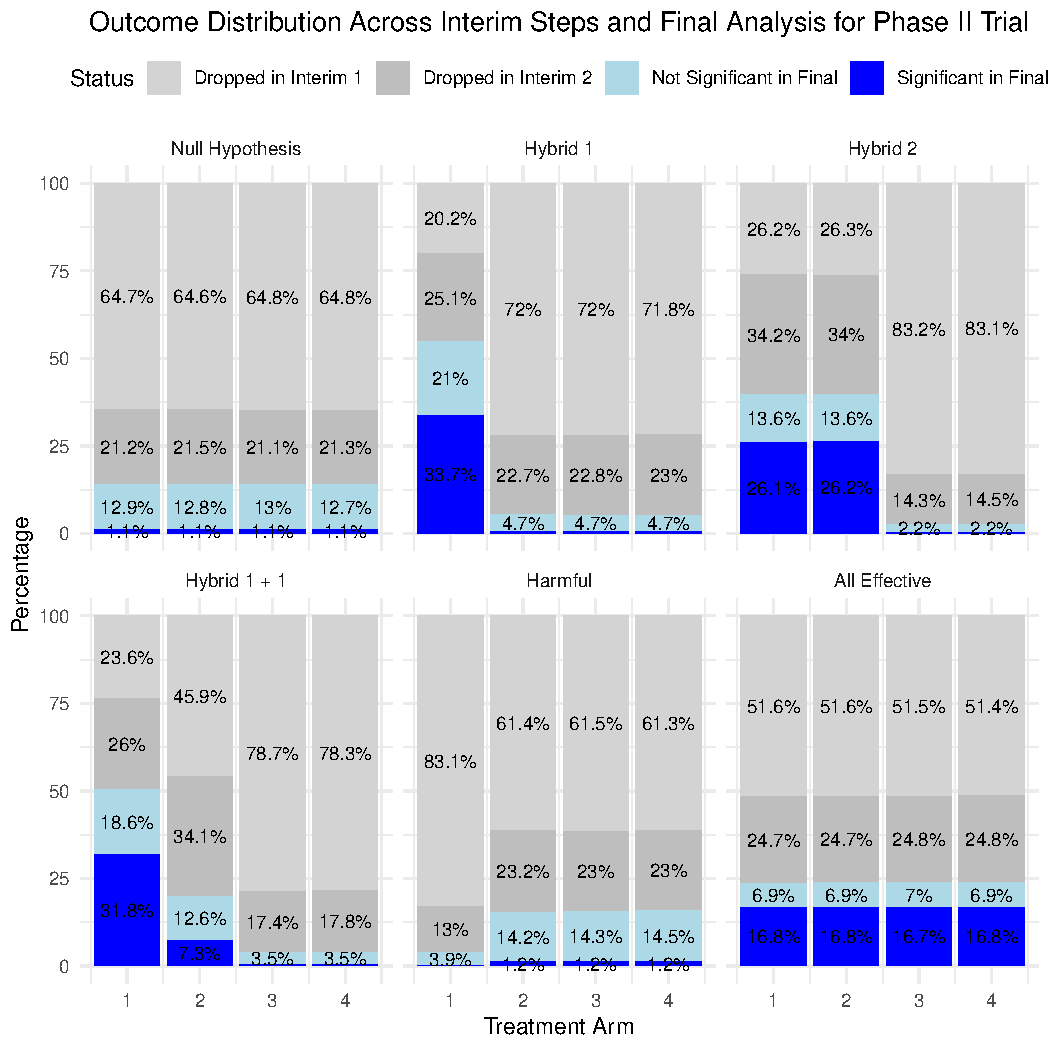
\includegraphics[width=\maxwidth]{figure/barplot_phase2_logrank-1} 

}


\end{knitrout}
    \caption{Outcome distribution across interim steps and final analysis for different scenarios for Phase II Trial. In the visualization, percentages below 1\% are omitted to improve clarity and avoid overcrowding, as such small values can make the chart difficult to interpret. However, for the Null Hypothesis, all percentages are displayed regardless of their size to ensure full visibility. Additionally, all results, including those below 1\%, are fully available in Table \ref{tab:outcome_distribution_phase2_appendix} for detailed examination.
}
    \label{fig:outcome_distribution_phase2_appendix}
\end{figure}


\begin{landscape}
% latex table generated in R 4.4.1 by xtable 1.8-4 package
% Sun Dec  8 20:03:40 2024
\begin{table}[ht]
\centering
\begin{tabular}{rrllll}
  \hline
Scenario & TreatmentArm & Dropped in Interim 1 & Dropped in Interim 2 & Not Significant in Final & Significant in Final \\ 
  \hline
  1 &   1 & 129466 (64.73\%) & 42485 (21.24\%) & 12.89\% (12.82\% ; 12.95\%) & 1.14\% (1.11\% ; 1.16\%) \\ 
    1 &   2 & 129221 (64.61\%) & 42957 (21.48\%) & 12.79\% (12.72\% ; 12.85\%) & 1.12\% (1.1\% ; 1.15\%) \\ 
    1 &   3 & 129654 (64.83\%) & 42195 (21.1\%) & 12.96\% (12.9\% ; 13.03\%) & 1.11\% (1.09\% ; 1.13\%) \\ 
    1 &   4 & 129658 (64.83\%) & 42598 (21.3\%) & 12.75\% (12.68\% ; 12.81\%) & 1.12\% (1.1\% ; 1.15\%) \\ 
   \hline 
  2 &   1 & 40375 (20.19\%) & 50156 (25.08\%) & 21.04\% (20.96\% ; 21.12\%) & 33.7\% (33.6\% ; 33.79\%) \\ 
    2 &   2 & 143931 (71.97\%) & 45471 (22.74\%) & 4.74\% (4.69\% ; 4.78\%) & 0.56\% (0.55\% ; 0.58\%) \\ 
    2 &   3 & 143947 (71.97\%) & 45625 (22.81\%) & 4.69\% (4.65\% ; 4.73\%) & 0.52\% (0.51\% ; 0.54\%) \\ 
    2 &   4 & 143555 (71.78\%) & 45938 (22.97\%) & 4.7\% (4.66\% ; 4.75\%) & 0.55\% (0.53\% ; 0.56\%) \\ 
   \hline 
  3 &   1 & 52361 (26.18\%) & 68371 (34.19\%) & 13.56\% (13.5\% ; 13.63\%) & 26.07\% (25.98\% ; 26.16\%) \\ 
    3 &   2 & 52515 (26.26\%) & 67955 (33.98\%) & 13.59\% (13.52\% ; 13.66\%) & 26.18\% (26.09\% ; 26.26\%) \\ 
    3 &   3 & 166434 (83.22\%) & 28633 (14.32\%) & 2.16\% (2.14\% ; 2.19\%) & 0.3\% (0.29\% ; 0.31\%) \\ 
    3 &   4 & 166113 (83.06\%) & 28971 (14.49\%) & 2.16\% (2.13\% ; 2.19\%) & 0.3\% (0.29\% ; 0.31\%) \\ 
   \hline 
  4 &   1 & 47258 (23.63\%) & 51965 (25.98\%) & 18.55\% (18.47\% ; 18.63\%) & 31.84\% (31.75\% ; 31.93\%) \\ 
    4 &   2 & 91863 (45.93\%) & 68264 (34.13\%) & 12.64\% (12.57\% ; 12.7\%) & 7.3\% (7.25\% ; 7.35\%) \\ 
    4 &   3 & 157375 (78.69\%) & 34779 (17.39\%) & 3.49\% (3.45\% ; 3.52\%) & 0.43\% (0.42\% ; 0.45\%) \\ 
    4 &   4 & 156604 (78.3\%) & 35528 (17.76\%) & 3.49\% (3.45\% ; 3.52\%) & 0.45\% (0.44\% ; 0.46\%) \\ 
   \hline 
  5 &   1 & 166164 (83.08\%) & 25945 (12.97\%) & 3.87\% (3.83\% ; 3.91\%) & 0.08\% (0.07\% ; 0.08\%) \\ 
    5 &   2 & 122878 (61.44\%) & 46334 (23.17\%) & 14.21\% (14.14\% ; 14.28\%) & 1.18\% (1.16\% ; 1.21\%) \\ 
    5 &   3 & 123039 (61.52\%) & 45996 (23\%) & 14.26\% (14.19\% ; 14.33\%) & 1.22\% (1.2\% ; 1.24\%) \\ 
    5 &   4 & 122557 (61.28\%) & 46022 (23.01\%) & 14.5\% (14.43\% ; 14.57\%) & 1.21\% (1.19\% ; 1.23\%) \\ 
   \hline 
  6 &   1 & 103168 (51.58\%) & 49487 (24.74\%) & 6.92\% (6.87\% ; 6.97\%) & 16.76\% (16.68\% ; 16.83\%) \\ 
    6 &   2 & 103105 (51.55\%) & 49481 (24.74\%) & 6.87\% (6.82\% ; 6.92\%) & 16.84\% (16.77\% ; 16.91\%) \\ 
    6 &   3 & 102913 (51.46\%) & 49576 (24.79\%) & 7.02\% (6.97\% ; 7.07\%) & 16.73\% (16.66\% ; 16.8\%) \\ 
    6 &   4 & 102898 (51.45\%) & 49617 (24.81\%) & 6.93\% (6.89\% ; 6.98\%) & 16.81\% (16.73\% ; 16.88\%) \\ 
   \hline 
 \hline
\end{tabular}
\caption{Outcome Distribution Across Interim Steps and Final Analysis in Phase II Trial (with 95\% Confidence Intervals for the Final Analysis).} 
\label{tab:outcome_distribution_phase2_appendix}
\end{table}

\end{landscape}


\begin{figure}[H]
    \centering
\begin{knitrout}
\definecolor{shadecolor}{rgb}{0.969, 0.969, 0.969}\color{fgcolor}

{\centering 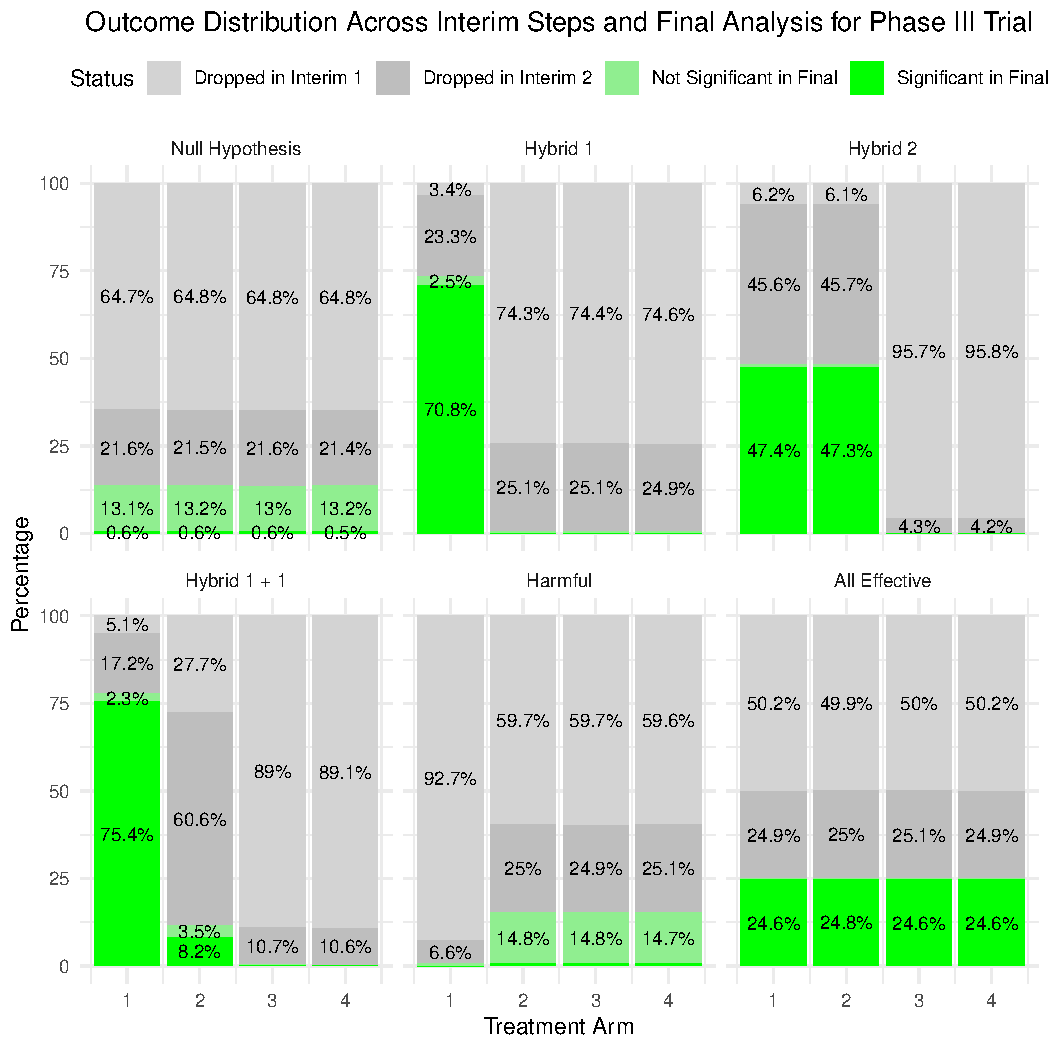
\includegraphics[width=\maxwidth]{figure/barplot_phase3_logrank-1} 

}


\end{knitrout}
    \caption{Outcome distribution across interim steps and final analysis for different scenarios for Phase III Trial. In the visualization, percentages below 1\% are omitted to improve clarity and avoid overcrowding, as such small values can make the chart difficult to interpret. However, for the Null Hypothesis, all percentages are displayed regardless of their size to ensure full visibility. Additionally, all results, including those below 1\%, are fully available in Table \ref{tab:outcome_distribution_phase3_appendix} for detailed examination.
}
    \label{fig:outcome_distribution_phase3_appendix}
\end{figure}


\begin{landscape}
% latex table generated in R 4.4.1 by xtable 1.8-4 package
% Sun Dec  8 20:04:17 2024
\begin{table}[ht]
\centering
\begin{tabular}{rrllll}
  \hline
Scenario & TreatmentArm & Dropped in Interim 1 & Dropped in Interim 2 & Not Significant in Final & Significant in Final \\ 
  \hline
  1 &   1 & 129445 (64.72\%) & 43255 (21.63\%) & 13.1\% (13.03\% ; 13.16\%) & 0.55\% (0.54\% ; 0.57\%) \\ 
    1 &   2 & 129552 (64.78\%) & 42913 (21.46\%) & 13.18\% (13.11\% ; 13.24\%) & 0.59\% (0.58\% ; 0.61\%) \\ 
    1 &   3 & 129688 (64.84\%) & 43196 (21.6\%) & 12.99\% (12.92\% ; 13.06\%) & 0.57\% (0.55\% ; 0.58\%) \\ 
    1 &   4 & 129647 (64.82\%) & 42847 (21.42\%) & 13.21\% (13.14\% ; 13.28\%) & 0.54\% (0.53\% ; 0.56\%) \\ 
   \hline 
  2 &   1 & 6829 (3.41\%) & 46600 (23.3\%) & 2.48\% (2.45\% ; 2.51\%) & 70.81\% (70.72\% ; 70.89\%) \\ 
    2 &   2 & 148654 (74.33\%) & 50275 (25.14\%) & 0.5\% (0.49\% ; 0.52\%) & 0.03\% (0.03\% ; 0.04\%) \\ 
    2 &   3 & 148770 (74.39\%) & 50173 (25.09\%) & 0.49\% (0.47\% ; 0.5\%) & 0.04\% (0.04\% ; 0.04\%) \\ 
    2 &   4 & 149150 (74.58\%) & 49743 (24.87\%) & 0.52\% (0.5\% ; 0.53\%) & 0.04\% (0.03\% ; 0.04\%) \\ 
   \hline 
  3 &   1 & 12394 (6.2\%) & 91116 (45.56\%) & 0.88\% (0.86\% ; 0.89\%) & 47.37\% (47.27\% ; 47.47\%) \\ 
    3 &   2 & 12236 (6.12\%) & 91434 (45.72\%) & 0.9\% (0.88\% ; 0.91\%) & 47.27\% (47.17\% ; 47.37\%) \\ 
    3 &   3 & 191359 (95.68\%) & 8528 (4.26\%) & 0.05\% (0.05\% ; 0.05\%) & 0.01\% (0.01\% ; 0.01\%) \\ 
    3 &   4 & 191577 (95.79\%) & 8325 (4.16\%) & 0.04\% (0.04\% ; 0.05\%) & 0\% (0\% ; 0.01\%) \\ 
   \hline 
  4 &   1 & 10123 (5.06\%) & 34477 (17.24\%) & 2.31\% (2.28\% ; 2.34\%) & 75.39\% (75.3\% ; 75.47\%) \\ 
    4 &   2 & 55474 (27.74\%) & 121170 (60.58\%) & 3.47\% (3.43\% ; 3.5\%) & 8.21\% (8.16\% ; 8.26\%) \\ 
    4 &   3 & 177922 (88.96\%) & 21469 (10.73\%) & 0.28\% (0.27\% ; 0.29\%) & 0.03\% (0.03\% ; 0.03\%) \\ 
    4 &   4 & 178297 (89.15\%) & 21138 (10.57\%) & 0.26\% (0.25\% ; 0.27\%) & 0.02\% (0.02\% ; 0.03\%) \\ 
   \hline 
  5 &   1 & 185318 (92.66\%) & 13245 (6.62\%) & 0.72\% (0.7\% ; 0.73\%) & 0\% (0\% ; 0\%) \\ 
    5 &   2 & 119406 (59.7\%) & 49914 (24.96\%) & 14.76\% (14.69\% ; 14.83\%) & 0.58\% (0.57\% ; 0.6\%) \\ 
    5 &   3 & 119475 (59.74\%) & 49722 (24.86\%) & 14.81\% (14.74\% ; 14.88\%) & 0.59\% (0.57\% ; 0.6\%) \\ 
    5 &   4 & 119214 (59.61\%) & 50188 (25.09\%) & 14.72\% (14.65\% ; 14.79\%) & 0.58\% (0.57\% ; 0.6\%) \\ 
   \hline 
  6 &   1 & 100429 (50.21\%) & 49834 (24.92\%) & 0.29\% (0.28\% ; 0.3\%) & 24.58\% (24.5\% ; 24.67\%) \\ 
    6 &   2 & 99808 (49.9\%) & 50033 (25.02\%) & 0.27\% (0.26\% ; 0.28\%) & 24.81\% (24.73\% ; 24.9\%) \\ 
    6 &   3 & 99999 (50\%) & 50201 (25.1\%) & 0.27\% (0.26\% ; 0.28\%) & 24.63\% (24.54\% ; 24.71\%) \\ 
    6 &   4 & 100379 (50.19\%) & 49860 (24.93\%) & 0.27\% (0.26\% ; 0.28\%) & 24.61\% (24.53\% ; 24.7\%) \\ 
   \hline 
 \hline
\end{tabular}
\caption{Outcome Distribution Across Interim Steps and Final Analysis in Phase II Trial (with 95\% Confidence Intervals for the Final Analysis).} 
\label{tab:outcome_distribution_phase3_appendix}
\end{table}

\end{landscape}




























\section{Personal Statement} \label{sec:statment}

I hereby declare that this master's thesis was independently conducted and written by me. Certain sections of the thesis have been proofread and corrected for spelling and grammar using generative AI tools. I take full responsibility for the content and affirm that all sources are properly cited.

\section{Reproducibility} \label{sec:app_reproducibility}

\flushleft{
This document was generated on December 08, 2024 at 20:04.
\textsf{R} version and packages used to generate this report see Subchapter \ref{sec:session_info}.
}

The complete code used for reproducibility in this project is available as open source in the GitHub repository linked below. To get started, please refer to the README file, which contains detailed instructions on how to set up the environment, run the code, and reproduce the results presented in this work.\\

Github Repository: \url{https://github.com/pfistem/BMS_Masterthesis}


\section{Session Info} \label{sec:session_info}
\begin{knitrout}
\definecolor{shadecolor}{rgb}{0.969, 0.969, 0.969}\color{fgcolor}\begin{kframe}
\begin{verbatim}
## 2024-12-08 20:04:17.561433 Europe/Zurich
## R version 4.4.1 (2024-06-14)
## Platform: x86_64-pc-linux-gnu
## Running under: Ubuntu 24.04.1 LTS
## 
## Matrix products: default
## BLAS:   /usr/lib/x86_64-linux-gnu/blas/libblas.so.3.12.0 
## LAPACK: /usr/lib/x86_64-linux-gnu/lapack/liblapack.so.3.12.0
## 
## locale:
##  [1] LC_CTYPE=en_GB.UTF-8       LC_NUMERIC=C              
##  [3] LC_TIME=en_GB.UTF-8        LC_COLLATE=en_GB.UTF-8    
##  [5] LC_MONETARY=en_GB.UTF-8    LC_MESSAGES=en_GB.UTF-8   
##  [7] LC_PAPER=en_GB.UTF-8       LC_NAME=C                 
##  [9] LC_ADDRESS=C               LC_TELEPHONE=C            
## [11] LC_MEASUREMENT=en_GB.UTF-8 LC_IDENTIFICATION=C       
## 
## time zone: Europe/Zurich
## tzcode source: system (glibc)
## 
## attached base packages:
## [1] stats     graphics  grDevices utils     datasets  methods   base     
## 
## other attached packages:
## [1] xtable_1.8-4  ggplot2_3.5.1 dplyr_1.1.4   knitr_1.48   
## 
## loaded via a namespace (and not attached):
##  [1] vctrs_0.6.5       cli_3.6.3         rlang_1.1.4       xfun_0.46        
##  [5] highr_0.11        generics_0.1.3    labeling_0.4.3    glue_1.7.0       
##  [9] colorspace_2.1-0  scales_1.3.0      fansi_1.0.6       grid_4.4.1       
## [13] evaluate_0.24.0   munsell_0.5.1     tibble_3.2.1      lifecycle_1.0.4  
## [17] compiler_4.4.1    pkgconfig_2.0.3   rstudioapi_0.16.0 farver_2.1.2     
## [21] tcltk_4.4.1       R6_2.5.1          tidyselect_1.2.1  utf8_1.2.4       
## [25] pillar_1.9.0      magrittr_2.0.3    tools_4.4.1       withr_3.0.0      
## [29] gtable_0.3.5
\end{verbatim}
\end{kframe}
\end{knitrout}

\newpage
\nocite{R}
\bibliographystyle{ims}
\bibliography{reference}
\vfill
\footnotesize

\end{document}
